%%%%%%%%%%%%%%%%%%%%%%%%%%%%%%%%%%%%%%%%%%%%%%%%%%%%%%%%%%%%%%%%%%%%%%%%%%%%
% diverse saker här som används i dokumentet %%%%%%%%%%%%%%%%%%%%%%%%%%%%%%%
\newcommand{\TitleText}{Radiohandbok HF}
\newcommand{\SubtitleText}{För Sändaramatörer, Privatradioanvändare\\
	och andra radiointresserade}
\newcommand{\Forfattare}{Täpp-Anders Sikvall}
\newcommand{\Initialer}{SM5UEI}
\newcommand{\DokYear}{19}
\newcommand{\DokVersion}{2.2.1-dev}
\newcommand{\DokumentRevision}{x.y.z}
\newcommand{\DokumentDatum}{\today}
%%%%%%%%%%%%%%%%%%%%%%%%%%%%%%%%%%%%%%%%%%%%%%%%%%%%%%%%%%%%%%%%%%%%%%%%%%%

%%%%%%%%%%%%%%%%%%%%%%%%%%%%%%%%%%%%%%%%%%%%%%%%%%%%%%%%%%%%%%%%%%%%%%%%%%%%
% diverse saker här som används i dokumentet %%%%%%%%%%%%%%%%%%%%%%%%%%%%%%%
\newcommand{\TitleText}{Radiohandbok}
\newcommand{\SubtitleText}{För Sändaramatörer\\ och Privatradioanvändare}
\newcommand{\Forfattare}{Täpp-Anders Sikvall}
\newcommand{\Initialer}{SMØUEI}
\newcommand{\DokYear}{19}
\newcommand{\DokVersion}{2.2.0}
\newcommand{\DokumentDatum}{2023-11-26}
%%%%%%%%%%%%%%%%%%%%%%%%%%%%%%%%%%%%%%%%%%%%%%%%%%%%%%%%%%%%%%%%%%%%%%%%%%%

\renewcommand{\arraystretch}{1.15}

\documentclass[10pt,swedish,a4paper]{article}
\usepackage[a4paper,bindingoffset=1cm]{geometry}
\usepackage[utf8]{inputenc}
\usepackage[T1]{fontenc}
\usepackage[swedish]{babel}
\usepackage[colorlinks,linkcolor=black,urlcolor=blue]{hyperref}
\usepackage{enumitem}
\usepackage{multirow}
\usepackage{amsmath}
\usepackage{tabularx}
\usepackage{graphicx}
\usepackage[table,x11names]{xcolor}
\usepackage{fancyhdr}
\usepackage[yyyymmdd]{datetime} \renewcommand{\dateseparator}{-}
\usepackage{lastpage}
%\usepackage{newpxtext,newpxmath}
\usepackage{pdfpages}
\usepackage{icomma}
\usepackage{pdflscape}
\usepackage{wrapfig}
\usepackage{float}
\usepackage[bottom]{footmisc}
\usepackage{longtable}
\usepackage{fbb}
\newif\iftitlefoot
\raggedbottom
\setlist{nosep}
\usepackage{todonotes}
\raggedbottom

\begin{document}
	
\newgeometry{left=2cm,right=2cm,bottom=1cm,top=1cm}
\pagestyle{empty}
\vfill
\vspace*{4cm}
\centerline{
\includegraphics[width=\paperwidth]{logo/rubrikbild}}
\begin{flushright}
	\Huge{\bfseries{\TitleText}} \\[3mm]
	\Large{\bfseries{\SubtitleText}}
\end{flushright}

\vfill
	
Version: \DokVersion\ \hfill SMØUEI \hfill Datum: \DokumentDatum

\newpage

\newgeometry{top=3cm}

\pagestyle{fancy}
\lhead{\leftmark}
\rhead{
	\scriptsize
	\begin{tabular}{ll}
		\textbf{Version} & \textbf{Datum}\\
		\ \DokVersion & \DokumentDatum\\
	\end{tabular}
}

\chead{}

\lfoot{
	\scriptsize
	www.sm0uei.se
}

\cfoot{\scriptsize \thepage\ / \pageref{LastPage}}

\rfoot{\scriptsize
	anders@sikvall.se
}

\renewcommand{\footrulewidth}{0.2pt}

\widowpenalty=9999
\clubpenalty=9999

%	\setlength{\headsep}{1em}2

\cleardoublepage

%%% Innehållsförteckning
\tableofcontents

\newpage

\setlength{\parskip}{0.5em}
\setlength{\parindent}{0pt}

\section*{Förord}
	
Detta är den uppdaterade utgåvan för november 2023. Det var ett tag
sedan som jag ägnade mig åt det här alstret och det har kommit in lite
påpekanden om rättningar och att repeaterlistor med mera varit ganska
utdaterade. Det är förstås helt riktigt och jag har i skrivande stund
faktiskt försökt få in den färskaste informationen som finns från SSA.

Mycket har hänt sedan föregående information. Jag har flyttat från
Stockholm och har numera blivit SM5UEI men hänger fortfarande på
Kvarnbergets amatörradioklubb på torsdagskvällarna så där är det öppet
hus dessa dagar från kl. 19:00 när ni alla är välkomna att kika förbi.

Ändringar som skett sedan förra utgåvan:

\begin{itemize}[]
	\item Landsprefixdelen har kortats av och delats upp lite enligt 
	input från SMØMPV.
	\item Bandplanerna har setts över, bl.a. 60\,m-bandet i HF-delen 
	har lagts till då det saknades tidigare.
	\item Repeaterlistan uppdaterad med senaste data från SSA
	\item Gjort om några exempel-QSO enligt tips från SMØMPV
	\item En hel hoper med uppsnyggningar och förbättringar här och där.
\end{itemize}

Bidrag till handboken tas tacksamt mot men jag kommer bedöma ifall
materialet är lämpligt att ta med.  Hela materialet finns numera också
på Github om man vill gräva i det och fixa-dona, komma med 
förbättrings\-förslag och annat kul så finns den på följande länk:

\href{https://github.com/sikvall/rhb/}{https://github.com/sikvall/rhb}

Har ni en massa bra förslag på grejer som ni skulle vilja ha med i boken
så låt mig veta det där, det går också om ni vill arbeta in ändringar direkt
och skicka mig en s.k. "pull request" så kan jag kika på det. Det går också
att logga issues om man hittar fel.

Och kör radio där ute. Mobilt. Stabilt. Maritimt. Aeromobilt. Alltid med
stil.\\[4em]

Karlholm, \DokumentDatum\\
\textit{Täpp-Anders Sikvall\\
	SM5UEI}

\clearpage
	

\section{Signaler och anrop}
\subsection{Landsprefix}

Här är inte alla länder med utan de vanligaste som körs från Sverige.

\begin{center}
\begin{longtable}{cl|cl}
	   	\caption{Tabell över landsprefix}\\
	   \textbf{Signal} & \textbf{Land}        & \textbf{Signal} & \textbf{Land}         \\ \hline
	   \endfirsthead
	\endhead
              AMA--AOZ     & Spanien              & C3A--C3Z        & Andorra               \\
	      C4A--C4Z     & Cypern               & DAA--DRZ        & Tyskland              \\
	      EAA--EHZ     & Spanien              & EIA--EJZ        & Irland                \\
	      EKA--EKZ     & Armenien             & EMA--EOZ        & Ukraina               \\
	      EBA--ERZ     & Moldav.              & ESA--ESZ        & Estland               \\
	      EUA--EWZ     & Vitryssland          & EXA--EXZ        & Ryssland              \\
	      EYA--EYZ     & Tajikistan           & EZA--EZZ        & Turkmenistan          \\
	      FAA--FZZ     & Frankrike            & GAA--GZZ        & Storbrittannien       \\
	      HAA--HZZ     & Ungern               & HBA--HBZ        & Schweiz               \\
	      HEA--HEZ     & Schweiz              & HFA--HFZ        & Polen                 \\
	      HGA--HGZ     & Ungern               & HVA--HVZ        & Vatikanen             \\
	      HWA--HYZ     & Frankrike            & H2A--H2Z        & Cypern                \\
	      IAA--IZZ     & Italien              & JWA--JXZ        & Norge                 \\
	      J4A--J4Z     & Grekland             & LAA--LNZ        & Norge                 \\
	      LXA--LXZ     & Luxemburg            & LYA--LYZ        & Litauen               \\
	      LZA--LZZ     & Bulgarien            & MAA--MZZ        & Storbrittannien       \\
	      OEA--OEZ     & Österrike            & OFA--OJZ        & Finland               \\
	      OKA--OLZ     & Tjeckiska republiken & OMA--OMZ        & Slovakiska republiken \\
	      ONA--OTZ     & Belgien              & OUA--OZZ        & Danmark               \\
	      PAA--PIZ     & Nederländerna        & P3A--P3Z        & Cypern                \\
	      RAA--RZZ     & Ryska federationen   & SAA--SMZ        & Sverige               \\
	      SNA--SRZ     & Polen                & TAA--TCZ        & Turkiet               \\
	      TFA--TFZ     & Island               & THA--THZ        & Frankrike             \\
	      TKA--TKZ     & Frankrikte           & TMA--TMZ        & Frankrike             \\
	      TOA--TQZ     & Frankrike            & TVA--TXZ        & Frankrike             \\
	      T9A--T9Z     & Bosnien-Herzegovina  & UAA--UIZ        & Ryska federationen    \\
	      UJA--UMZ     & Uzbekistan           & UNA--UQZ        & Kazakstan             \\
	       URA-UTZ     & Ukraina              & UUA--UZZ        & Ukraina               \\
	      VPA--VSZ     & Storbritannien       & XPA--XPZ        & Danmark               \\
	      XXA--XXZ     & Portugal             & YLA--YLZ        & Litauen               \\
	      Y2A--Y9Z     & Tyskland             & ZBA--ZJZ        & Storbritannien        \\
	      ZNA--ZOZ     & Storbritannien       & ZQA--ZQZ        & Storbritannien        \\
	       2AA-2ZZ     & Storbritannien       & 3YA--3YZ        & Norge                 \\
	      3ZA--3ZZ     & Polen                & 5BA--5BZ        & Cypern                \\
	      5PA--5QZ     & Danmark              & 7SA--7SZ        & Sverige               \\
	      8SA--8SZ     & Sverige              & 9AA--9AZ        & Kroatien
\end{longtable}
\end{center}

\subsection{Svenska signaler}

Svenska signaler förekommer inom ett antal prefix. Enligt ITU disponerar Sverige förljande signalserier: 7SA--7SZ samt 8SA--8SZ och vidare de mer kända SAA--SMZ. Dessa har används till varierande ändamål, exempelvis har flyget signaler i serien SE-AAA--ZZZ. Polisen har tidigare använt signaler i serien SHA plus fyra siffror, detta är nu ersatt med nytt system i.o.m. RAKEL. Räddningstjänsten använde SDA med fyra siffror. Signaler som 7SA + 4 siffror används för mindre yrkesbåtar SC + 4 siffror för fritidsbåtar.

Amatörradion använder ett antal signaler, de viktigaste är:

\begin{tabular}{ll}
	SM & Amatörradiosignal utdelad av PTS (nya signaler tilldelas ej i serien) \\
	SA & Amatörradiosignal tilldelad av SSA, ESA eller FRO                     \\
	SK & Klubbsignaler (som regel tvåställiga efter distriktsiffran)           \\
	SL & Militära signaler (som regel tvåställiga efter distriktsiffran)
\end{tabular}

Dessa signaler följs av en \textit{distriktsiffra} se särskilt avsnitt och sedan 2-ställiga eller 3-ställiga bokstavskombinationer som är den personliga signalen. Exempel är SM0UEI som är min egen signal, distriktsiffran är 0 dvs hemmavarande i Stockholms län. Ett annat exempel kan vara SK5JV tidigare Fagersta amatörradioklubb.

Repeatrar som tillhör klubbar får ofta signal efter klubben med tillägg /R för repeater.

Det finns numera även ett stort antal signaler som är tillfälliga eller knutna till särskilda event, exempelvis scoutverksamhet som ibland sänder amatörradio och särskilda forskningsfartyg, flyg- och rymdfart mm.

Som suffix används följande:

\begin{tabular}{ll}
	/M  & Mobil (rörlig) sändaramatör, även portabel \\
	/MM & Mobil till sjöss (mobil maritime)          \\
	/AM & Mobil i luften (aeromobile)                \\
	/PM & Mobil portabel (ej officiellt suffix)\\
	/R  & Repeaterstation
\end{tabular}

\subsection{Svenska distrikten}

Sverige delas in i följande distrikt efter sina län:

\begin{table}[h]
	\centering
\begin{tabular}{cl}
	\textbf{Distrikt} & \textbf{Län}                                     \\ \hline %\endhead
	      0        & Stockholm                                        \\
	      1        & Gotland                                          \\
	      2        & Västerbotten, Norrbotten                         \\
	      3        & Gävleborg, Jämtland, Västernorrland              \\
	      4        & Örebro, Värmland, Dalarna                        \\
	      5        & Östergötland, Södermanland, Västmanland, Uppsala \\
	      6        & Halland, Västra götaland                         \\
	      7        & Skåne, Blekinge, Kronoberg, Jönköping, Kalmar    \\
	      8        & Speciella stationer utanför landets gränser
\end{tabular}
\caption{Distriktssiffor i Sverige}
\end{table}
Distrikten förekommen som siffra i utdelade anropssignaler. Radioamatörer byter inte distriktsiffra under resa i annat distrikt, i stället används suffix (tillägg efter ordinarie signal) som t.ex. /M för mobil. Ofta uppger man "SM0UEI mobilt i SM3-land" för att påvisa att man befinner sig utanför ordinarie distrikt.

I de tidigare SMnXYZ-signalerna förekom amatörens bokstavskombination endast en gång, det kunde alltså inte finnas en SM4UEI och en SM0UEI, det vore i så fall samma amatör som flyttat. Med det nya systemet där SSA m.fl. utdelar signaler i stället för PTS i serien SAnXYZ kan SM4XYZ och SA7XYZ alltså vara två helt olika amatörer.
\section{Terminologi och trafik}

\subsection{Bokstaveringsalfabetet (Svenska)}

\begin{table}[H]
	\centering
\begin{longtable}{cl|cl|cl }
	A & Adam   & O & Olof    & 1 & Ett        \\
	B & Bertil & P & Petter  & 2 & Tvåa       \\
	C & Cesar  & Q & Qvintus & 3 & Trea       \\
	D & David  & R & Rudolf  & 4 & Fyra       \\
	E & Erik   & S & Sigurd  & 5 & Femma      \\
	F & Filip  & T & Tore    & 6 & Sexa       \\
	G & Gustav & U & Urban   & 7 & Sju        \\
	H & Helge  & V & Viktor  & 8 & Åtta       \\
	I & Ivar   & W & Wilhelm & 9 & Nia        \\
	J & Johan  & X & Xerxes  & 0 & Nolla      \\
	K & Kalle  & Y & Yngve   & . & Punkt      \\
	L & Ludvig & Z & Zäta    & , & Komma      \\
	M & Martin & Å & Åke     & - & Minus      \\
	N & Niklas & Ä & Ärlig   & + & Plus       \\
	  &        & Ö & Östen   &   & Mellanslag \\
\end{longtable}
\caption{Svenska bokstaveringsalfabetet}
\end{table}

\subsection{Bokstaveringsalfabetet (Internationella)}
\begin{table}[H]
\centering
\begin{tabular}{cl|cl|cl}
	A & Alfa     &  P   & Papa       & 0 & Zero    \\
	B & Bravo    &  Q   & Quebec     & 1 & One     \\
	C & Charlie  &  R   & Romeo      & 2 & Two     \\
	D & Delta    &  S   & Sierra     & 3 & Tree    \\
	E & Echo     &  T   & Tango      & 4 & Fower   \\
	F & Foxtrot  &  U   & Uniform    & 5 & Fife    \\
	G & Golf     &  V   & Victor     & 6 & Six     \\
	H & Hotel    &  W   & Whiskey    & 7 & Seven   \\
	I & India    &  X   & X-ray      & 8 & Ait     \\
	J & Juliet   &  Y   & Yankee     & 9 & Niner   \\
	K & Kilo     &  Z   & Zulu       & . & Stop    \\
	L & Lima     & Å/AA & Alfa-Alfa  & , & Decimal \\
	M & Mike     & Ä/AE & Alfa-Echo  & - & Minus   \\
	N & November & Ö/OE & Oscar-Echo & + & Plus    \\
	O & Oscar    &      &            &   & Space   \\
\end{tabular}
\caption{Internationella bokstaveringsalfabetet (ITU-alfabetet)}
\end{table}

\subsection{Q-koder}
\begin{longtable}{ll}
	\textbf{Kod} & \textbf{Fråga / Svar}                                                         \\ \hline \endhead
	QRA & Vad heter er station?                                                \\
	    & Vår station heter ...                                                \\ \hline
	QRB & Hur långt bort från min station befinner ni er?                      \\
	    & Avståndet mellan oss är ungefär ...                                  \\ \hline
	QRG & Kan ni ange min exakta frekvens?                                     \\
	    & Er exakta frekvens är ... (MHz/kHz)                                  \\ \hline
	QRH & Varierar min frekvens/våglängd?                                      \\
	    & Er frekvens/våglängd varierar.                                       \\ \hline
	QRI & Hur är min sändningston (CW)?                                        \\
	    & Er sändningston är 1--God, 2--Varierande, 3--Dålig                   \\ \hline
	QRK & Vilken uppfattbarhet har mina signaler?                              \\
	    & Uppfattbarheten hos dina signaler är:                                \\
	    & 1--Dålig, 2--Bristfällig, 3--Ganska god, 4--God, 5--Utmärkt          \\ \hline
	QRL & Är ni upptagen?                                                      \\
	    & Jag är upptagen med ... (namn/signal) stör ej.                       \\ \hline
	QRM & Är ni störd av annan station?                                        \\
	    & Störningarna är:                                                     \\
	    & 1--Obef., 2--Svaga, 3--Måttliga, 4--Starka, 5--Mycket starka         \\ \hline
	QRN & Besväras ni av atmosfäriska störningar?                              \\
	    & Störningarna är:                                                     \\
	    & 1--Obef., 2--Svaga, 3--Måttliga, 4--Starka, 5--Mycket starka         \\ \hline
	QRO & Kan jag (ska jag) öka sändareffekten?                                \\
	    & Öka sändareffekten.                                                  \\ \hline
	QRP & Kan jag (ska jag) minska sändareffekten?                             \\
	    & Minska sändareffekten.                                               \\ \hline
	QRQ & Kan jag (får jag) öka sändningshastigheten?                          \\
	    & Öka sändningshastigheten.                                            \\ \hline
	QRS & Kan jag (skall jag) sända långsammare?                               \\
	    & Sänd långsammare.                                                    \\ \hline
	QRT & Skall jag avbryta sändningen?                                        \\
	    & Avbryt sändningen                                                    \\ \hline
	QRU & Har ni något till mig?                                               \\
	    & Jag har inget till er. Se även QTC.                                  \\ \hline
	QRV & Är ni redo?                                                          \\
	    & Jag är redo.                                                         \\ \hline
	QRX & När anropar ni mig härnäst?                                          \\
	    & Jag anropar er kl ... (på ... MHz/kHz)                               \\ \hline
	QRZ & Vem anropar mig?                                                     \\
	    & Ni anropas av ... (på ... MHz/kHz).                                  \\ \hline
	QSA & Vilken styrka har mina signaler?                                     \\
	    & Era signaler är:                                                     \\
	    & 1--Ej uppf., 2--Svaga, 3--Ganska starka, 4--Starka, 5--Mycket starka \\ \hline
	QSB & Svajar styrkan på mina signaler?                                     \\
	    & Styrkan på era signaler svajar.                                      \\ \hline
	QSK & Kan du höra mig mellan dina tecken och får jag avbryta dig?          \\
	    & Jag kan höra dig mellan mina tecken och du får avbryta.              \\ \hline
	QSL & Kan ni ge mig kvittens?                                              \\
	    & Jag kvitterar.                                                       \\ \hline
	QSO & Ha ni förbindelse med ... eller ... (förmedlat)?                     \\
	    & Jag har förbindelse med ... (via ...)                                \\ \hline
	QST & Har tidigare använts som allmänt anrop men ersatts av CQ             \\ \hline
	QSY & Skall jag övergå till att sända på annan frekvens?                   \\
	    & Gå över till att sända på annan frekvens (eller ... kHz/MHz).        \\ \hline
	QTC & Hur många telegram har ni att sända?                                 \\
	    & Jag har ... telegram till dig (eller ...).                           \\ \hline
	QTH & Vilken är er geografiska position?                                   \\
	    & Min geografiska position är ...                                      \\ \hline
	QTR & Kan ni ge mig rätt tid?                                              \\
	    & Rätt tid är ...                                                      \\ \hline
\end{longtable}

\subsection{Lokator}

Lokator (Maidenhead locator) är ett praktiskt sätt att tala om sin ungefärliga position genom att ange endast sex stycken tecken. En lokator kan t.ex. se ut som JO89VK vilket täcker in nordvästa Järfälla. Det finns många verktyg för att räkna på lokator där ute, det är bra att känna sin egen. Det finns appar för detta till telefonerna som både kan räkna på bäring, distans mellan två rutor och dessutom via telefonens GPS bestämma vilken lokator du för närvarande befinner dig i.

Första paret dela in jorden i 18x18 fält, dvs 20 grader per fält longitud och 10 grader per fält latitud. Varje sådant fält delas sedan in i 10x10 rutor som numreras 0-9 på vardera axeln. Dessa i sin tur delas sedan in i 24x24 smårutor som då får storleksordningen 2.5 grader latitud och 5 grader long. vardera.

\subsection{Uppträdande}

När vi kör amatörradio finns det ett antal saker att tänka på som har att göra med hur vi beter oss mot varandra på banden. Se detta som en guide till hur man bör uppträda på banden.

En radioamatör måste vara \textbf{tolerant}. Vi delar frekvenser med många andra personer, en del av dem kommer inte ha samma uppfattning som du själv har om saker och ting. Här gäller det att vara tolerant, förstående och framför allt inte bli upprörd över personer som kanske inte beter sig som du önskade att de betedde sig.

Radioamatörer är \emph{aldrig ensamma på banden} helt oavsett om någon svarar på ditt allmänna anrop eller ej så finns det i det närmaste \textbf{garanterat någon som lyssnar}. 

Tänk på vad du säger och att du undviker diskutera ämnen som kan verka \textbf{upprörande} eller \textbf{stötande}. Ämnen som bör undvikas är \textbf{religion} och livs\-å\-skå\-d\-ni\-ng, \textbf{politisk} ideologi, \textbf{ekonomiska} eller \textbf{sociala} frågor m.m. där motparter kan ha starka åsikter som inte nödvändigtvis stämmer med dina egna. Radion är inte ett agitationsrum för sådana frågor.

\textbf{Svordomar}, \textbf{könsord} och liknande undviker vi helt. Språket skall vara vårdat men behöver inte vara strikt. Tänk på att din motpart är inte den enda som lyssnar utan det finns \textit{andra amatörer som lyssnar}, icke-amatörer som lyssnar, myndigheter som lyssnar och så vidare.

Ha \textbf{förståelse} för att andra kanske inte har dina egna detaljkunskaper, professionalism med mera. Agera \textbf{ödmjukt} gentemot andra människor på banden.

Blir du ändå upprörd, undvik att \emph{agera på det} över huvud taget. Sänd inte över annans sändning, s.k. ''gummitumme'', eller stör på annat vis för du är upprörd. Avsluta hellre QSO:t, byt frekvens eller återkom lite senare när du lugnat ned dig. Tänk på att \textit{de flesta konflikter orsakas av okunskap eller brist på förståelse}. \textbf{Agera vuxet} i sådana situationer och jobba för att \textbf{de-eskalera} situationen.

En skicklig amatör \textit{lyssnar mycket innan sändning}. Vi anropar på ett korrekt sätt och avslutar på ett korrekt sätt. Vi försöker uppge våra respektive signaler på ett \emph{tydligt och läsligt sätt}, i dag finns det en tendens att sluddra över signalerna framför allt på 2m och 70cm banden, gör inte det. Tydlighet är en vinning i sig. 

När någon ny i ringen inträder, räkna upp de deltagande signalerna så att personen tydligt får en bild av alla som är med och vem som är på turen före och efter hen.

Vi pratar inte \textbf{nedvärderande} om personer varesig de är andra amatörer eller ej, eller en viss grupp av personer. Vi undviker \textbf{sexuella anspelningar} och vitsar ''\textbf{under bältet}'' liksom allt för \textbf{personliga detaljer}. Amatörradion är främst för \textbf{tekniska diskussioner} av rent \textbf{privat natur} eller av \textbf{allmänt intresse för hobbyn}, tester och prov med mera.

Undvik väldigt \textbf{långa sändningspass}. Ibland händer det saker hos dina motstationer som att de får ett viktigt telefonsamtal eller måste springa ut i köket för katten har rivit ner något, ett barn ramlar eller annat som gör att man måste kvickt lämna radion. Att \textbf{långprata} i sådana lägen gör det svårt att tala om ''QRX --- jag måste ta hand om en sak, anropar dig igen om 5 min.''. Enstaka gånger kanske man behöver förklara något lite längre men gör det till en vana att lämna luckor så ofta som möjligt.

\textbf{Nödtrafik har alltid prioritet} och måste respekteras på alla
frekvenser.

\subsection{Repeatrar}

Repeatrars syfte är främst att förlänga kommunikationen från mobila och portabla amatörsändare. Samtal mellan fasta stationer förekommer men om ni hör varandra på direkten, övergå gärna till en simplex-frekvens i stället för att belägga repeatern.

Lämna luckor mellan er när ni växlar station som sänder. Gör det möjligt för andra att ''breaka-in'' särskilt om ert QSO fortsätter under längre tid. Ta hänsyn till att andra kanske vill använda repeatern för att nå personer som de inte kan nå annars. Hänsyn åt båda hållen förutsätts här. 

Repeatern är en begränsad resurs. Det är inte okay att lägga beslag på den under långa perioder när andra kanske behöver den, var ödmjuk inför att någon driver repeatern och har satt upp den i första hand för att supporta mobila stationer.

Nödtrafik har alltid prioritet.

\subsection{QSO}

Konsten att genomföra ett radiosamtal (QSO) i olika sammanhang.

\subsubsection{Radiosamtalets delar}

Ett radiosamtal består som regel av tre delar. Först sker ett anrop, när kontakt etablerats utväxlas ett antal meddelande (dialog) och när man är klarar avslutas samtalet. Dessa tre delar är ganska standard. Man följer detta ganska strikt t.ex. på kortvågen där telefoni oftast innebär SSB. Anledningen är enkel, det går inte höra när någon släpper sändtangenten eller bara är tyst och tänker.

När man kör FM över repeatrar på VHF/UHF är det inte lika vanligt att man både öppnar och avslutar varje sändning med motparten och sin egen signal. Men man skall regelbundet upprepa signalerna och i praktiken är det lämpligt att göra kanske var femte minut eller oftare.

\subsubsection{Anropet}

Ett anrop kan se ut ungefär såhär:

<<<<<<< HEAD
--- SM0MAD från SM0UEI, SA0MAD kom!
=======
--- SA0MAD från SM0UEI, SA0MAD kom!
>>>>>>> 9b0d699b43f86e40d49f75e6dd4d94047b3fe129

Här är det SA0MAD som anropas av SM0UEI. 

<<<<<<< HEAD
=======
Svaret kan se ut ungefär såhär:

>>>>>>> 9b0d699b43f86e40d49f75e6dd4d94047b3fe129
--- SM0UEI från SA0MAD kom!

Därefter övergår radiosamtalet i dialog eller meddelandesändning.

\subsubsection{Allmänt anrop} 

Används när man inte ropar på någon särskild motstation utan önskar samtal med vem som helst. På svenska använder man ofta just orden ''allmänt anrop'' medan på engelska är det vanligare att man uttalar CQ (seek you). Ett allmänt androp kan se ut såhär:

--- Allmänt anrop, allmänt anrop, allmänt androp från SM0UEI SM0UEI SM0UEI kallar allmänt anrop och lyssnar.

Eller på engelska:

--- CQ CQ CQ this is SM0UEI calling CQ CQ CQ and standing by.

\subsubsection{Meddelandesändning}

--- SA0MAD från SM0UEI, tack för svaret. Din signal är 59 hos mig, mitt QTH är JO89WA och namnet är Anders. SA0MAD från SM0UEI kom.

--- SM0UEI från SA0MAD, tack för rapporten. Din signal är 57 hos mig, jag befinner mi i JO89VK men kommer under kvällen byta QTH. Jag kommer då vara QRV på 3663 kHz. QSL? SM0UEI från SA0MAD.

--- SA0MAD från SM0UEI, QSL på det, QRX 19.30 på frekvens 3663 kHz. 

\subsubsection{Avslutning}

--- SA0MAD från SM0UEI, tack för rapport och vi hörs senare, 73, slut kom

--- SM0UEI från SA0MAD, 73 tillbaka, klart slut.

\subsection{Contest}

Under contest är det vanligtvis så att man kör ett relativt kort QSO för att hinna så många som möjligt. Under constestförhållanden utväxlar man som regel signal, sekvensnummer, signalrapport med varandra. Ofta lägger man till "contest" i sitt anrop exempelvis:

--- CQ Contest CQ Contest CQ Contest SM0UEI SM0UEI CQ Contest

Efter man etablerat kontakt utväxlar man signalrapporter och sekvensnummer

--- SM0UEI from SA0MAD, you are 59 here and sequence 28, SM0UEI from SA0MAD.

--- SA0MAD from SM0UEI, QSL your signals are 58 and my sequence is 112, QSL? SA0MAD from SM0UEI

--- QSL and good luck, SM0UEI from SA0MAD

\subsubsection{Pile-up}

Ibland kan det bli väldigt många motstationer samtidigt som ropar. Nu gäller det att spetsa öronen! Först gäller det att sålla. Rara signaler från långtbortistan ger mer poäng i en contest som regel eller från länder du inte kört osv beroende på regler. Försök att sålla med "du som sänder från Florida" eller "VK7 kom igen" osv till det är en station kvar. Kör den snabbt, ropa CQ igen och börja sålla.

Direkt när det uppstår en pile-up är det effektivt att köra split. Dvs du lyssnar 5-10 kHz upp eller ned från den frekvens du sänder på. Det gör det lättare för dig att behålla kommandot under pile-up. Ligger du och sänder i ett frekvensområde som är särskilt ägnat för DX är det smart att lägga Rx-frekvensen strax utanför. Det undviker att man stökar ned i DX-bandet.

Kör du split skall du säga det efter varje sändning. "CQ CQ CQ de Sierra Mike Zeor Uniform Echo India listening 5 up" exempelvis. På CW bör en split vara minst 2 kHz och på SSB bör den vara minst 5 kHz ännu hellre 10 kHz. Tänk på att när du startar din split måste du kolla så att båda frekvenserna är ok. Låt inte din pile-up sprida ut sig för mycket även om det är kanske enklare för dig så är risken stor att den stör någon annan. 

Kör korta QSO. Utbyt snabbt den information som behövs och ta sedan nästa. Ha förståelse för att det kan bli krockar i en pile-up. När du hör en partiell signal eller station du vill prata med håll fast vid den. Om du har svårt att läsa den be den repetera tills ni är klara. Genom att du är auktoriteten på frekvensen kommer pile-up:en att lugna ned sig och vänta på sin tur. Om du ''hattar omkring'' är risken att all radiodisciplin far ut genom fönstret.

Använd ett standardmönster när du kör:

--- SM0UEI CQ CQ CQ de SM0UEI 10 UP

--- SM0UEI de ON3XYZ you are 59 sequence 122, QSL?

--- ON3XYZ SM0UEI QSL, 59 back to you, sequence 312 QSL?

--- QSL. CQ CQ CQ de SM0UEI 10 UP ...

Om du försöker nå en motstation med pile-up var uppmärksam på dennes sändningar och vänta på din tur. Tala gärna om signal och var du sänder från men släpp sedan fram andra. Tänk på hur du själv skulle vilja att en pile-up på din egen station skulle vilja agera. Den gyllene regeln är också alltid lyssna först --- sänd sedan!


\section{Teknik}

\subsection{Effekt i dBW och dBm}

Effekter anges i W eller i decibel relaterat till 1 mW (dBm) eller relaterat 1W (dBW). Tabell över effekt och decibelwatt nedan:
\begin{table}[h]
\begin{tabular}{rrr|rrr|rrr}
	\textbf{Effekt} & \textbf{dBW} & \textbf{dBm} & \textbf{Effekt} & \textbf{dBW} & \textbf{dBm} & \textbf{Effekt} & \textbf{dBW} & \textbf{dBm} \\ \hline
	    1 \textmu W &          -60 &          -30 &             1 W &            0 &           30 &           100 W &           20 &           50 \\
	   10 \textmu W &          -50 &          -20 &             3 W &            5 &           35 &           250 W &           24 &           54 \\
	  100 \textmu W &          -40 &          -10 &             5 W &            7 &           37 &           500 W &           27 &           57 \\
	           1 mW &          -30 &            0 &            10 W &           10 &           40 &            1 kW &           30 &           60 \\
	          10 mW &          -20 &           10 &            20 W &           13 &           43 &          1.5 kW &           32 &           62 \\
	         100 mW &          -10 &           20 &            50 W &           17 &           47 &          2.0 kW &           33 &           63
\end{tabular}
\caption{Tabell över effekt och decibelskalor}
\end{table}

\subsection{S-värden, signalvärde, S-meter}

Signalstyrkan i amatörradio uttrycks oftast som S-värden. Dessa fås i regel genom nivån på AGC hos mottagaren. Därför ser man sälla utslag vid riktigt låga signaler.

Standard kalibrering för S-metern är enligt skalan i tabellen \ref{tab:s-varden}

\begin{table}[h]
\begin{tabular}{r|rr|rr||r|rr|rr}
      & \multicolumn{2}{c|}{\textbf{$<$ 30 MHz}} &
  \multicolumn{2}{c}{\textbf{$>$ 30 MHz}}       && \multicolumn{2}{c|}{\textbf{$<$ 30 MHz}} &
  \multicolumn{2}{c}{\textbf{$>$ 30 MHz}}\\ \textbf{S} & \textbf{dBm}
  & \textbf{\textmu V} & \textbf{dBm} & \textbf{\textmu V}&   \textbf{S} & \textbf{dBm}
  & \textbf{\textmu V} & \textbf{dBm} & \textbf{\textmu V} \\\hline
          
	   1 & -121 & 0.21  & -141 & 0.02 & 9+10 & -63 & 160  & -83 & 16  \\
	   2 & -115 & 0.40  & -135 & 0.04 & 9+20 & -53 & 500  & -73 & 50  \\
	   3 & -109 & 0.80  & -129 & 0.08 & 9+30 & -43 & 1600 & -63 & 160 \\
	   4 & -103 & 1.60  & -123 & 0.16 & 9+40 & -33 & 5000 & -53 & 500 \\
	   5 & -97  & 3.20  & -117 & 0.32 &      &     &      &     &     \\
	   6 & -91  & 6.30  & -111 & 0.63 &      &     &      &     &     \\
	   7 & -85  & 12.60 & -105 & 1.26 &      &     &      &     &     \\
	   8 & -79  & 25.00 & -99  & 2.50 &      &     &      &     &     \\
	   9 & -73  & 50.00 & -93  & 5.00 &      &     &      &     &     \\
\end{tabular}
\caption{Tabell över S-värden, effekt och spänning}
\label{tab:s-varden}
\end{table}

\subsection{Modulationer}

\subsubsection{Bandbredd olika modulationer}

Olika modulationer upptar olika bandbredd. Detta är mycket viktigt att förstå när man ställer in sin radiostation. Detta gäller särskilt att beakta i närheten av nödfrekvenser eller bandkanten. När vi talar om bandbredder här förstås den bandbredd vari minst 98\% av signalens effekt befinner sig.

\begin{tabular}{lrl}
	\textbf{Modulation} & \textbf{Bandbredd} & \textbf{Kommentarer}                  \\ \hline
	CW                  &          $<$500 Hz & Smalbandigt                           \\
	AM                  &              6 kHz & Amplitudmodulering med fullt sidband  \\
	SSB*                &              <3 kHz & Amplitudmodulering med enkelt sidband \\
	NFM                 &           7-12 kHz & Smalbandig FM                         \\
	FM                  &             16 kHz & Normal FM                             \\
	WFM                 &          16-75 kHz & Bredbandig FM (t.ex. rundradio)
\end{tabular}

*) För SSB gäller att USB och LSB fungerar lite olika. När man beräknar den högsta eller lägsta frekvensen utgår man från den inställda frekvensen $f$. För USB gäller då att högsta frekvensen är $f+3$\,kHz. För LSB blir det $f-3$\,kHz. Detta innebär att om du sänder på 80\,m-bandet och du får sända telefoni från 3600--3800\,kHz och vill lägga dig i under bandkanten och köra LSB skall du ställa in din radio på 3603\,kHz som lägsta frekvens. Använd gärna lite marginal och kör exempelvis 3605\,kHz i stället.

Den egentliga modulationsfrekvensen är dock lite mer komplicerad. Normalt anges den verkliga modulationsfrekvensen som ca 2,7\,kHz och det beror på att man i regel filtrerar bort ljudet under 300\,Hz och det över 3000\,Hz. Detta innebär att det akustiska frekvensomfånget blir 300--3000\,Hz och därmed upptar signalen inte mer än 2,7\,kHz.

Det är vanligt att man märker stationer som kör överdriven bandbredd. Antingen som en följd av att man vill öka sin modulationsvinst, okunskap eller man har skruvat i sin radio. Syftet kan var att få bättre genomslag vid långväga förbindelser.

\subsubsection{Telegrafi, CW}

CW står för continuous waves och innebär en rent omodulerad bärvåg. I mottagaren används en oscillator för att återskapa hörbar signal. Detta används för telegrafi och modulationsslaget är oftast A1A. Ibland sänds telegrafi som modulerad AM-bärvåg också som då moduleras med t.ex. 700\,Hz ton. Det är dock mindre vanligt.

Bandbredden för CW är i teorin mycket smal. I praktiken blir den lite beroende på frekvens från några Hz till något hundratal Hz beroende på frekvensband och sändarens beskaffenhet i form av jitter och frekvensstabilitet.

Bandbredden hos CW består av fasbruset vilket normalt är så undertryckt att det egentligen inte betyder så mycker samt stig- respektive falltiden när man nycklar eller släpper nyckeln. Sker detta mjukt är bandbredden låg, har man skarp in- eller urkoppling av bärvågen nyttjar man mer bandbredd.

\subsubsection{Amplitudmodulering, AM}

Amplitudmodulering finns i flera olika varianter. Vanlig AM består av en bärvåg vars styra varieras i takt med signalen som skall sändas. Denna förändring av bärvågen producerar sidband och det är i dessa som den egentliga informationen återfinns. Bärvågen i sig får dock lejonparten av signalen varför det är en sändningsklass som nästan aldrig används inom amatörradiobanden.

Bandbredden hos AM-modulerad signal kan beräknas genom att man tar två gånger högsta modulationsfrekvensen. Detta ger t.ex. vid en modulationsfrekvens som går från 300-3000\,Hz en bandbredd som varierar med talet från upp till 6\,kHz.

$$B=2f_m$$

Där $f_m$ är högsta modulationsfrekvensen.

\subsubsection{SSB/ESB -- Enkelt sidband, en AM-variant}

Enkelt sidband används av radioamatörer för att minska på bandbredden samt lägga radioenergin där den behövs mest. Eftersom båda sidbanden innehåller samma information kan man filtrera bort dessa samt bärvågen innan man matar sändarens förstärkarsteg med resultatet. I mottagaren behöver man dock återskapa en referenssignal, en så kallad beat-oscillator gör detta. När man ställer in frekvensen så försöker man därmed matcha den ursprungliga frekvensen. Ligger man för långt från låter det kalle anka, kommer man för nära sidbandet låter det dovt och basigt. 

Enkelt sidband förkortas ESB eller SSB (single side-band) och man kan välja vilket sidband man vill använda sig av. På amatörradiofrekvenser under 10 MHz använder man LSB (lägre/lower sidbandet) och på frekvenser över 10 MHz används USB/ÖSB (upper/övre sidbandet). 

Detta är mycket av tradition. Använder man fel sorts sidband hörs det inget vettigt när man försöker lyssna. Språkrytmerna gör dock att vi uppfattar det som att mänskligt tal förekommer. I dag händer det att amatörer bryter mot regeln och sänder med ``fel'' sidband på fel frekvens.

Bandbredden hos SSB är halva den för normal AM egentligen. Den kan därmed beräknas som för AM och halveras.

$$B=f_m$$

Där $f_m$ är högsta modulationsfrekvensen.

\subsubsection{Frekvensmodulering, FM}

Frekvensmodulering består av att man tar en bärvåg och modulerar den med talet genom att skifta dess frekvens. Om skiftet i frekvens är mycket litet kallas moduleringen för fasmodulation. FM-modulering indelas i lite olika klasser beroende på hur stor deviation som används. På amatörradions VHF- och UHF-band talar vi om FM och NFM (Narrow FM, andra namn förekommer också). Ibland talar man om bred FM, normal FM och smal FM på svenska.

Normal FM innebär att deviationen (hur mycket signalen avviker från grundfrekvensen) är lika stor som den högsta modulationsfrekvensen. Det är vanligt att kommunikationsradio använder sig av 3 kHz som högsta modulationsfrekvens och 5 kHz deviation. Deviationen är då något bredare och ger upphov till en viss modulationsvinst. När man talar om FM-radio på UKV-bandet för rundradio så är deviationen ca 75\,kHz och högsta modulationsfrekvens ca 16\,kHz. Där är alltså svinget betydligt bredare än modulationen och detta är bred FM.

Nu för tiden förordas en minskning av bandbredden för FM-sändningar på amatörbanden, främst är det väl VHF och UHF där FM-sändning är vanligast förekommande och där vill man ha en kanalindelning om 12,5\,kHz i stället för som tidigare 25\,kHz. Om man studerar bandbredden hos olika FM-signaler kan man använda sig av Carsons bandbreddsbegrepp:

$$B=2(f_M+f_D)$$

Där $B$ är bandbredden $f_M$ högsta modulationsfrekvensen och $f_d$ är FM-signalens maximala deviation (även kallat sving). Carsons bandbreddsbegrepp säger att 98\% av energin förekommer inom den stipulerade bandbredden. Det betyder att att grannkanalen kan få ungefär 17\,dB lägre signal under sändning vilket fortfarande inte är enormt bra. Carson var för övrigt den som faktiskt uppfan SSB-modulationen.

\begin{center}
\begin{tabular}{rrrr}
Deviation & Modulation & Bandbredd & Kanaldelning\\ \hline
5 kHz & 3 kHz & 16 kHz & 25 kHz\\
2.5 kHz & 3 kHz & 11 kHz & 12.5 kHz\\
\end{tabular}
\end{center}

\subsection{Termiska brusgolvet}

\begin{center}
\begin{tabular}{rr|rr|rr}
	\textbf{RBW} & \textbf{N$_0$} & \textbf{RBW} & \textbf{N$_0$} & \textbf{RBW} & \textbf{N$_0$} \\ \hline
	         0.5 &           -141 &         6.25 &           -136 &          100 &           -124 \\
	         1.0 &           -144 &        12.50 &           -133 &          200 &           -121 \\
	         3.0 &           -139 &        25.00 &           -130 &         5000 &           -107 \\
	         5.0 &           -137 &        50.00 &           -127 &        10000 &           -104
\end{tabular}
\end{center}

Mottagarbandbredden (RBW) anges i kHz och brusgolvet i dBm (dB relaterat en styrka om 1 mW).

\subsection{Return loss och VSWR}

Return loss och VSWR anger samma sak. VSWR är vanligare inom amatörradio medan man i profesionella sammanhang föredrar att prata om return loss. RL är storleken på den reflekterade signalen i förhållande till den framåtgående signalen. Return loss mäts alltså i dB enligt formeln $10\log(P_F/P_R)$ där $P_F$ är den framåtgående effekten (forward) och  $P_R$ är den reflekterade signalen i retur.

\begin{longtable}{rrr|rrr|rrr}
	\textbf{RL} & \textbf{VSWR} & \textbf{\%} & \textbf{RL} & \textbf{VSWR} & \textbf{\%} & \textbf{RL} & \textbf{VSWR} & \textbf{\%} \\ \hline 	\endhead
	          1 &         17,39 &       79,43 &           8 &          2,32 &       15,85 &          20 &          1,22 &        1,00 \\
	          2 &          8,72 &       63,10 &          10 &          1,92 &       10,00 &          22 &          1,17 &        0,63 \\
	          3 &          5,85 &       50,12 &          12 &          1,67 &        6,31 &          24 &          1,13 &        0,40 \\
	          4 &          4,42 &       39,81 &          14 &          1,50 &        3,98 &          25 &          1,12 &        0,32 \\
	          5 &          3,57 &       31,62 &          15 &          1,43 &        3,16 &          26 &          1,11 &        0,25 \\
	          6 &          3,01 &       25,12 &          16 &          1,38 &        2,51 &          28 &          1,08 &        0,16 \\
	          7 &          2,61 &       19,95 &          18 &          1,29 &        1,58 &          30 &          1,07 &        0,10
\end{longtable}

Acceptabelt RL är ungefär från 12\,dB, riktigt bra från 20 dB och de bästa komponenterna ligger runt 30\,dB. Många antenntuners som går med automatik startar avstämningen först när VSWR är 1:2 eller sämre som motsvarar ca 10\,dB\,RL.

\subsection{CTCSS subtoner}

Inom amatörradio används ofta pilottoner (subtoner) som CTCSS\footnote{Contnuous Tone-Conded Squelch System} för repeatrar och liknande. På PMR446 används subtoner för att skapa virtuella grupper och sub-kanaler. De som används är följande toner och frekvenser:

\begin{tabular}{rr|rr|rr|rr|rr}
	 1 &  67,0 &  2 &  69,3 &  3 &  74,4 &  4 &  77,0 &  5 &  79,7 \\ \hline
	 6 &  82,5 &  7 &  85,4 &  8 &  88,5 &  9 &  91,5 & 10 &  94,8 \\ \hline
	11 &  97,4 & 12 & 100,0 & 13 & 103,5 & 14 & 107,2 & 15 & 110,9 \\ \hline
	16 & 114,8 & 17 & 118,8 & 18 & 123,0 & 19 & 127,3 & 20 & 131,8 \\ \hline
	21 & 136,5 & 22 & 141,3 & 23 & 146,2 & 24 & 151,4 & 25 & 156,7 \\ \hline
	26 & 162,2 & 27 & 167,9 & 28 & 173,8 & 29 & 179,9 & 30 & 186,2 \\ \hline
	31 & 192,8 & 32 & 203,5 & 33 & 210,7 & 34 & 218,1 & 35 & 225,7 \\ \hline
	36 & 233,6 & 37 & 241,8 & 38 & 250,3 &    &       &    &
\end{tabular}

\subsection{CTCSS-zoner i Sverige}

Rekommendationer för repeatrar i olika distrikt och län att använda CTCSS för att hindra att störningar uppkommer vid conds mm. Det ger också möjligheten för sändaramatörer att öppna just den repeater man önskar om man har flera på samma frekvens omkring sig.

\begin{tabular}{lcccc}
	\textbf{Område}    & \textbf{Primär} & \textbf{Sek. 1} & \textbf{Sek. 2} & \textbf{Sek. 3} \\ \hline
	Distrikt 0         & 77,0            & 123.0           & 67.0            & 100.0           \\
	Distrikt 1         & 218.1           & 233.6           &                 &                 \\
	Distrikt 2         & 107.2           & 146.2           & 162.2           & 186.2           \\
	Distrikt 3         & 127.3           & 141.3           & 250.3           &                 \\
	D4 Värml. / Örebro & 74.4            & 151.4           &                 &                 \\
	D4 Dalarna         & 85.4            & 151.4           &                 &                 \\
	Distrikt 5         & 82.5            & 91.5            & 103.5           & 203.5           \\
	Distrikt 6         & 114.8           & 118,8           & 94.8            & 131.8           \\
	Distrikt 7         & 79.7            & 156.7           & 210.7           & 
\end{tabular}

Lägg märke till att decimalsiffran är i de flesta fall samma som distriktssiffran.

\section{Bandbredd olika modulationer}

Olika modulationer upptar olika bandbredd. Detta är mycket viktigt att förstå när man ställer in sin radiostation. Detta gäller särskilt att beakta i närheten av nödfrekvenser eller bandkanten. När vi talar om bandbredder här förstås den bandbredd vari minst 98 \% av signalens effekt befinner sig.

\begin{tabular}{lrl}
	\textbf{Modulation} & \textbf{Bandbredd} & \textbf{Kommentarer}                  \\ \hline
	CW                  &          $<$500 Hz & Smalbandigt                           \\
	AM                  &              6 kHz & Amplitudmodulering med fullt sidband  \\
	SSB*                &              3 kHz & Amplitudmodulering med enkelt sidband \\
	NFM**               &           7-12 kHz & Smalbandig FM                         \\
	FM                  &             16 kHz & Normal FM                             \\
	WFM                 &          16-75 kHz & Bredbandig FM (t.ex. rundradio)
\end{tabular}

*) För SSB gäller att USB och LSB fungerar lite olika. När man beräknar den högsta eller lägsta frekvensen utgår man från den inställda frekvensen $f$. För USB gäller då att högsta frekvensen är $f+3$ kHz. För LSB blir det $f-3$ kHz. Detta innebär att om du sänder på 80m bandet och du får sända telefoni från 3600--3800 kHz och vill lägga dig i under bandkanten och köra LSB skall du ställa in din radio på 3603 kHz som lägsta frekvens. Använd gärna lite marginal och kör exempelvis 3605 kHz i stället.

*) På kortvågen används smalbandig FM med max 10 kHz modulationsbandbredd. På VHF/UHF är smalbandig FM ca 11 kHz bred med Carssons bandbreddsbegrepp.

Det är vanligt att t.ex. utländska stationer kör överdriven bandbredd. Antingen som en följd av att man vill öka sin modulationsvinst, okunskap eller man har skruvat i sin radio.

\section{Övergripande frekvensplan}

\subsection{Indelning efter frekvens och våglängd}
\label{frekvens-vaglangd}

\begin{tabular}{llrlrl}
	\textbf{Förk.} & \textbf{Benämning}   & \textbf{Frekvens} &     & \textbf{Våglängd} &  \\ \hline
	ELF            & Extremt låg frekvens &             3--30 & Hz  &           10--100 & Mm \\
	SLF            & Superlåg frekvens    &           30--300 & Hz  &             1--10 & Mm \\
	ULF            & Ultralåg frekvens    &         300--3000 & Hz  &         100--1000 & km \\
	VLF            & Väldigt låg frekvens &             3--30 & kHz &           10--100 & km \\
	LF (LV)        & Låg frekvens         &           30--300 & kHz &             1--10 & km \\
	MF (MV)        & Mellanfrekvens       &         300--3000 & kHz &         100--1000 & m  \\
	HF (KV)        & Högfrekvens          &             3--30 & MHz &             1--10 & m  \\
	VHF (UKV)      & Väldigt hög frekvens &           30--300 & MHz &             1--10 & m  \\
	UHF            & Ultrahög frekvens    &         300--3000 & MHz &         100--1000 & mm \\
	SHF            & Superhög frekvens    &             3--30 & GHz &           10--100 & mm \\
	EHF            & Extremt hög frekvens &           30--300 & GHz &             1--10 & mm \\
	THF            & Terahertsfrekvens    &          300-3000 & GHz &         100--1000 & µm
\end{tabular}

Benämningarna HF, MF och LF har också andra betydelser. Exempelvis an\-vänd\-s HF som beteckning av den signal en antenn tar mot eller sänder oavsett frekvensband, MF kan vara mellansignalen oavsett frekvens efter omvandling i en superheterodynmottagare och LF, ibland benämnt AF (audiofrekvens) är det hörbara ljudet, dvs den modulation som används på signalen.

På engelska används i stället benämningarna RF för radio frequency, IF för intermediate frequency and AF för audio frequency vilket rekommenderas då sammanblandningsrisk med ITU-benämningarna på spektrum inte föreligger.

Amatörradioband finns inom de flesta av dessa frekvensband utom de högsta och lägsta frekvenserna.

\subsection{Rundradiobenämningar och frekvensband}

\begin{tabular}{llrl}
\textbf{Förk.} & \textbf{Namn} & \textbf{Frekvens Rundradio} &     \\ \hline
LW/LV          & Långvåg       & 148,5--285                  & kHz \\
MW/MV          & Mellanvåg     & 526,5--1606,5               & kHz \\
SW/KV          & Kortvåg       & 4,3--30                     & MHz \\
UKV            & Ultrakortvåg  & 88--108                     & MHz \\
\end{tabular}

\subsection{Radarband och benämningar enligt ITU}

\begin{tabular}{lrl}
	\textbf{Band} & \textbf{Frekvens} & \textbf{Benämning}          \\ \hline
	HF            &   0.003--0.03 GHz & High frequency              \\
	VHF           &     0.03--0.3 GHz & Very hgh frequency          \\
	UHF           &        0.3--1 GHz & Ultra high frequency        \\
	L             &          1--2 GHz & Long wave                   \\
	S             &          2--4 GHz & Short wave                  \\
	C             &          4--8 GHz &  \\
	X             &         8--12 GHz & Anv. under 2:a världskriget \\
	Ku            &        12--18 GHz & ''Kurz under''              \\
	K             &        18--27 GHz & Tyska ''Kurz'' (kortvåg)    \\
	Ka            &        27--40 GHz & Kurz-above (över)           \\
	V             &        40--75 GHz &  \\
	W             &       75--110 GHz &  \\
	mm            &      110--300 GHz & Millimetervågor
\end{tabular}

\subsection{Egenskaper olika frekvensband}

För radioamatörer delar man in frekvensbanden i långvåg, mellanvåg, kortvåg, VHF, UHF och SHF beroende på frekvens, se tabellen under avsnitt \ref{frekvens-vaglangd}. Dessa har lite olika utbredningsegenskaper.

\textbf{Långvåg} -- Markvågsutbredning, relativt höga sändareffekter, tillförlitliga för\-bind\-el\-ser men i övre delen av frekvensbandet kortare förbindelser dagtid. På de lägsta frekvenserna erhålls med hög sändareffekt goda förbindelser på stora avstånd globalt och används även för t.ex. malmprospektering, kommunikation med ubåtar i undervattensläge.

\textbf{Kortvåg} -- God rymdvågsutbredning med mycket lång räckvidd redan med låg effekt men samtidigt starkt avhängigt radiokonditionerna. Med ökande frekvens blir jonosfärreflektionen allt flackare vilket resulterar i en alltmer uttalad död zon (skip). Särskilt utmärkande för kortvågen är att den redan med låg effekt ger under gynnsamma konditioner extremt lång räckvidd via rymdvåg, ibland globalt.

\textbf{Mellanvåg} -- Kombinerar egenskaperna hos angränsande delar av lång- och kortvåg, kan ge kraftig interferens mellan rymd- och markvåg som ofta upplevs som kraftig fädning. Särskilt utmärkande för mellanvågen är den i det närmaste avsaknanden av skipzon eftersom mark- och rymdvåg kompletterar varandra, jonosfärens D-skikt är heller inte särskilt uttalat i frekvensområdet dvs förbindelser via rymdvåg på korta avstånd mellan 100--300\,km är möjliga även dagtid under perioder med kraftig solaktivitet.

\textbf{Ultrakortvåg (VHF)} -- Förbindeleser med låg effekt och små antenner, oberoende av jonosfären men då endast i form av frirumsutbredning, dvs fram till horisonten och under påverkan av terränghinder mm. Särskilt utmärkande för UKV är att rymdvåg saknar, markvågsdämpningen till lands är total och kommunikation på högre frekvenser i princip därför bara sker vid fri sikt mellan sändare och mottagare.


\clearpage

\section{Trafik- och tumregler HF}
\subsection{Kort sammanfattning av reglemente}

OBS! Detta är inte fullständigt radioreglemente naturligtvis utan endast sammanfattning av några viktiga punkter.

\subsubsection{Begrepp i bandplanerna}

\begin{itemize}
\item QRP: Aktivitetscentrum för låg effekt ($<$5W), svaga signaler förekommer, visa hänsyn.
\item QRS: Aktivitetscenter för långsam CW.
\item QRSS: Extremt långsam CW med dator.
\item DV: Digital Voice.
\item Image: Bildmoder exempelvis SSTV och Fax som ryms inom den specificerade maximala bandbredden.
\end{itemize}

\subsubsection{Trafikregler och tumregler}

\begin{itemize}
\item Vid SSB-telefoni används LSB på frekvenser under 10 MHz och USB på frekvenser över 10 MHz.
\item Lägsta acceptabla inställda frekvens för LSB är 3 kHz över under bandkant! 
\item Högsta acceptable inställda frekvens för USB är 3 kHz under övre bandkant!
\item IBP är International Beacon Project. Fyrarna sänder med 3 min intervaller och används för att studera utbredningen av radiosignaler globalt. Fyrarna sänder anrop och fyra 1 s toner. Anropet och första tonen sänds med 100W, därefter sänds tonerna med 10W, 1W samt 100mW.
\item Vid AM (A3J) skall hänsyn tas så att störningar på annan trafik ej fö\-re\-kom\-mer med de sidband som då uppstår, det gäller då både övre och undre sidbandet.
\item Ingen som helst sändning är tillåtet inom fyrsegmenten. Detta skall respekteras. Lyssna gärna på nödfrekvenserna men används dem icke, om det inte är du som svarar på ett nödsamtal! Undvik QSO allt för nära dessa också.
\item Var särskilt uppmärksam på satelliters nerlänksfrekvenser på 10\,m-bandet. I detta segment skall endast lyssning ske. Ingen sändning är tillåten här eller i skyddssegmentet strax ovanför satellitsegmentet. Tänk på att satelliters frekvens kan dopplerskiftas uppåt en hel del när de rör sig mot mottagaren.
\end{itemize}

\section{Frekvenser HF}

\subsection{PR-bandet 27\,MHz}

Detta är det enda bandet som allmänheten kan använda på HF-bandet. Det delar många egenskaper med 31\,MHz jaktradiobandet men är ett band som är äldre och mer etablerat.

Maximal uteffekt på bandet är 4W RMS ERP dvs antennvinst överstigande en 1/2-vågs dipol (0 dBd, 2.12 dBi) måste inräknas i effekten efter avdrag för matningsförlust. Modulationsslag AM, FM och SSB (primärt används USB) är tillåtet på alla kanaler i dag. Traditionellt används kanal 24 för USB men i dag får vilken kanal som helst användas.

Kanalerna med A efter är upplåtna för radiostyrning och inte för telefoni. Undvik därför att använda dessa om du har en sändare som kan använda dessa frekvenser. De är med i tabellen för den skall vara komplett. 

\clearpage

\begin{longtable}{rrl|rrl}
	\textbf{Frekvens}& \textbf{Kanalnr}& \textbf{Övrigt}        
	& \textbf{Frekvens} & \textbf{Kanalnr} & \textbf{Övrigt}  \\
	\hline \endhead
	  26,965 &       1 &                &   27,215 &      21 &          \\
	  26,975 &       2 &                &   27,225 &      22 &          \\
	  26,985 &       3 &                &   27,255 &      23 &          \\
	  26,995 &      3A & Radiostyrning  &   27,235 &      24 & SSB      \\
	  27,005 &       4 &                &   27,245 &      25 &          \\
	  27,015 &       5 &                &   27,265 &      26 &          \\
	  27,025 &       6 &                &   27,275 &      27 &          \\
	  27,035 &       7 &                &   27,285 &      28 &          \\
	  27,045 &      7A & Radiostyrning  &   27,295 &      29 &          \\
	  27,055 &       8 &                &   27,305 &      30 &          \\
	  27,065 &       9 &                &   27,315 &      31 &          \\
	  27,075 &      10 &                &   27,325 &      32 &          \\
	  27,085 &      11 &                &   27,335 &      33 &          \\
	  27,095 &     11A & Tid. nödfrekv. &   27,345 &      34 &          \\
	  27,105 &      12 &                &   27,355 &      35 &          \\
	  27,115 &      13 &                &   27,365 &      36 &          \\
	  27,125 &      14 &                &   27,375 &      37 &          \\
	  27,135 &      15 &                &   27,385 &      38 &          \\
	  27,155 &      16 &                &   27,395 &      39 &          \\
	  27,165 &      17 &                &   27,405 &      40 &          \\
	  27,175 &      18 &                &          &         &          \\
	  27,185 &      19 &                &          &         &          \\
	  27,195 &     19A & Radiostyrning  &          &         &          \\
	  27,205 &      20 &                &          &         &        
\end{longtable}

Många apparater är endast FM i dag men det finns de som också har SSB. Äldre apparater hade oftast AM och FM och ibland även SSB. Telegrafi körs i princip inte på PR-bandet, troligen för att det aldrig varit några krav på det och de som kör heller inte haft möjlighet förr i tiden att DX-a på bandet. 

Innan Televerket släppte upp bestämmelserna var det väldigt hårda bestämmelser på bandet, i princip var det bara kommunikation inom familjen som tilläts. I dag kan bandet användas som man vill och det är på sina håll god aktivitet. 

Kom ihåg att inte överskrida effektbegränsningarna bara.

\subsection{JOTA---Jamboree on the air, scoutfrekvenser}

Scouterna har frekvenser på HF likväl som VHF/UHF som de aktiverar vid särskilda tillfällen ofta i tillsammans med en lokal amatörradioklubb eller vanliga amtörradioeldsjälar som inte sällan också är scouter. Här kommer en lista på frekvenser som är vanligt förekommande i scoutsammanhang.

\begin{tabular}{rrll}
	\textbf{Band} & \textbf{Frekvens} & \textbf{Trafik} & \textbf{Not} \\ \hline

                   80 & 3 570  & CW  &             \\
	              & 3 940  & SSB & Ej region 2 \\
	              & 3 690  & SSB &             \\ \hline
	           40 & 7 030  & CW  &             \\
	              & 7 190  & SSB &             \\
	              & 7 090  & SSB &             \\ \hline
	           20 & 14 060 & CW  &             \\
	              & 14 290 & SSB &             \\ \hline
	           17 & 18 080 & CW  &             \\
	              & 18 140 & SSB &             \\ \hline
	           15 & 21 140 & CW  &             \\
	              & 21 360 & SSB &             \\ \hline
	           12 & 24 910 & CW  &             \\
	              & 24 960 & SSB &             \\ \hline
	           10 & 28 180 & CW  &             \\
	              & 28 390 & SSB &             \\ \hline
	            6 & 10 160 & CW  &             \\
	              & 50 160 & SSB &             \\ \hline
\end{tabular}

Normalt aktiveras dessa frekvenser tredje veckoslutet i oktober varje år, fredag till söndag. Då kan det vara många klubbar som finns på frekvenserna och det är också vanligt att man hör dem på helt andra frekvenser. De frekvenser som listas här är inte på något vis de endra frekvenser som scouter använder.

\subsection{Marina MF/HF-frekvenser}

De marina HF-banden är uppdelade på ett antal band. Det finns en generell kanalindelning med 3 kHz per kanal och SSB som modulationssätt på respektive band. Marina HF-kanaler finns på banden 4, 6, 8, 12, 16, 18, 22 och 25 MHz. 

MF även benämnd gränsvåg i marina sammanahang är inte lika ofta används som den var en gång i tiden. Nedan listas de frekvenser som används i Sverige.

\subsubsection{Svenska MF-kanaler}

\begin{longtable}{llrr}
\textbf{Kanal} & \textbf{Placering} & \textbf{Skepp} & \textbf{Kust}  \\ \hline 
\endhead

MF1 & Gotland       & 2 099 & 1 6874 \\
MF2 & ---           & ---  & ---   \\
MF3 & Gislövshammar & 2 060 & 1 797  \\
MF4 & Härnösand     & 2 216 & 2 733  \\
MF5 & Bjuröklubb    & 2 123 & 1 779  \\
MF6 & Grimeton      & 2 135 & 1 710
\end{longtable}

\subsubsection{Nödfrekvenser}

\begin{longtable}{lrr}
\textbf{Band} & \textbf{Frekvens} & \textbf{DSC Frekvens}\\ \hline \endhead

MF   & 2 182  & 2 187.5  \\
HF4  & 4 125  & 4 207.5  \\
HF6  & 6 215  & 6 312.0  \\
HF8  & 8 291  & 8 414.5  \\
HF12 & 12 290 & 12 577.0 \\
HF16 & 16 429 & 16 804.5 \\
\end{longtable}

\subsubsection{Primära HF skepp-till-skepp}

\begin{longtable}{lrrrrrrrr}
\textbf{Kanal} & \textbf{HF4} & \textbf{HF6} & \textbf{HF8} & \textbf{HF12} & \textbf{HF16} & \textbf{HF18} & \textbf{HF22} & \textbf{HF25} \\
\hline
\endhead

A & 4 146 & 6 224 & 8 294 & 12 353 & 16 528 & 18 825 & 22 159 & 25 100 \\
B & 4 149 & 6 227 & 8 297 & 12 356 & 16 531 & 18 828 & 22 162 & 25 103 \\
C &       & 6 230 &       & 12 359 & 16 534 & 18 831 & 22 165 & 25 106 \\
D &       &       &       & 12 362 & 16 537 & 18 834 & 22 168 & 25 109 \\
E &       &       &       & 12 365 & 16 540 & 18 837 & 22 171 & 25 112 \\
F &       &       &       &        & 16 543 & 18 840 & 22 174 & 25 115 \\
G &       &       &       &        & 16 546 & 18 843 & 22 177 & 25 118 \\
\end{longtable}

\clearpage
\subsection{Fyrar}

\subsubsection{IBP -- International Beacon Project}

Det finns flera olika typer av fyrar men för HF är IBP (International Beacon Project) intressant eftersom det ger operatören möjlighet att utröna hur utbredningen ser ut för stunden genom att lyssna efter fyrar. 

Fyrarna har gemensam hårdvara och synkroniseras mot tidsreferens. Fyrar kan vara offline av olika skäl, kontrollera mot IBP:s hemsida om du inte hör en fyr du brukar höra, den kan vara off line.

Tabellen nedan visar anropssignaler och första sändningsslotten som fyren sänder, dvs SCHED för olika fyrar och frekvenser.

\subsubsection{Lista över IBP-fyrar}
\small
\begin{tabular}{llrrrrr}
\textbf{Signal} & \textbf{QTH} & \textbf{14 100} & \textbf{18 110} & \textbf{21 150} & \textbf{24 930} & \textbf{28 200} \\ \hline

4U1UN  & United Nations & 00:00  & 00:10  & 00:20  & 00:30  & 00:40  \\ 
VE8AT  & Canada         & 00:10  & 00:20  & 00:30  & 00:40  & 00:50  \\
W6WX   & United States  & 00:20  & 00:30  & 00:40  & 00:50  & 01:00  \\
KH6RS  & Hawaii         & 00:30  & 00:40  & 00:50  & 01:00  & 01:10  \\
ZL6B   & New Zealand    & 00:40  & 00:50  & 01:00  & 01:10  & 01:20  \\
VK6RBP & Australia      & 00:50  & 01:00  & 01:10  & 01:20  & 01:30  \\
JA2IGY & Japan          & 01:00  & 01:10  & 01:20  & 01:30  & 01:40  \\
RR9O   & Russia         & 01:10  & 01:20  & 01:30  & 01:40  & 01:50  \\
VR2B   & Hong Kong      & 01:20  & 01:30  & 01:40  & 01:50  & 02:00  \\
4S7B   & Sri Lanka      & 01:30  & 01:40  & 01:50  & 02:00  & 02:10  \\
ZS6DN  & South Africa   & 01:40  & 01:50  & 02:00  & 02:10  & 02:20  \\
5Z4B   & Kenya          & 01:50  & 02:00  & 02:10  & 02:20  & 02:30  \\
4X6TU  & Israel         & 02:00  & 02:10  & 02:20  & 02:30  & 02:40  \\
OH2B   & Finland        & 02:10  & 02:20  & 02:30  & 02:40  & 02:50  \\
CS3B   & Madeira        & 02:20  & 02:30  & 02:40  & 02:50  & 00:00  \\
LU4AA  & Argentina      & 02:30  & 02:40  & 02:50  & 00:00  & 00:10  \\
OA4B   & Peru           & 02:40  & 02:50  & 00:00  & 00:10  & 00:20  \\
YV5B   & Venezuela      & 02:50  & 00:00  & 00:10  & 00:20  & 00:30  \\
\end{tabular}

\normalsize

\clearpage

\subsection{Olika trafiksätt på HF}

De olika HF-banden har olika egenskaper över tid på dagen, tid på året och påverkas vädligt mycket av rådande rymdväder och hur joniserat den övre delen av atmosfären är för att bilda rymdvåg.

Med det stora antalet band som radioamatörer förfogar över så finns det ofta något band som fungerar. Det gäller att man lär sig hur de olika egenskaperna påverkar de olika banden och när man kan förvänta sig att de ''öppnar'' och fungerar på längre avstånd.

Klassiska amatörradioband på kortvågen är därför 160 meter (som ju egentligen är ett gränsvågsband då det ligger precis under kortvågen enligt rådande ITU-definition), 80, 40, 60, 20, 17, 15, 12 och 10 metersbanden ger radioamatörer en stor karta av olika band att arbeta med.

För den som inte är radioamatör så är urvalet mer begränsat och även den effekt man lagligen får använda. Här finns egentligen bara 27~MHz och till nöds kan man väl även räkna jaktfrekvenserna på 31~MHz också men begränsningen i användandet och vilken effekt som står till buds gör att kortvågen är radioamatörernas jaktmark i första hand.

Vi ska i det här kapitlet titta lite på de olika bandens olika egenskaper och lite olika sätt att använda dem för att nå lokalt, lite längre och DX -- dvs i det närmaste globalt.

\subsubsection{Solens inverkan -- rymdvädret}

En sak som har mycket kraftig inverkan på radiosamband på kortvåg är rymdvädret. Som många känner till så följer solens solfläckar en 11-årig cykel och just nu inväntar vi toppen på cykel nummer 25 (numrerad från 1 sedan man började numrera dem) och dess topp förväntas inträffa under 2025. Därefter kommer vi se en nedgång i solfläckar fram till början av nästa cykel, som då blir cykel 26. 

I botten på solfläckscyklerna blir det ofta sämre så kallade konditioner på kortvågsbanden. Det blir svårare att nå långt och hitta ''öppningar'' på banden med högre frekvens, framför allt 15-, 12- och 10-metersbanden. Lokalt fungerar de bra men för de där riktiga DX-öppningarna behövs lite solaktivitet.

I toppen på solcykeln kan det däremot vara väldigt varierande. Ena dagen har man enorma öppningar på 10-metersbandet så att man kan kommunicera lokalt, men risken för en kraftig så kallad ''flare'' från solen eller en CME (koronal mass-utkasning, Coronal Mass Ejection) där en del av solens yta slungas iväg i kraftiga explosioner påverkar inte bara solvindens möjligheter att jonisera de övre luftlagren utan kan också skapa störningar i det jordmagnetiska fältet.

När detta sker brukar det åtföljas av kraftiga och vackra polarsken (norrksen i norr och sydsken i syd) och amatörerna benämner dessa som ''aurora''. Då denna uppträder är ofta kortvågen kraftigt påverkad på ett negativt sätt men ibland kan man nyttja själva auroran och studsa lite högre frekvenser på den som t.ex. VHF och då exempelvis 6-metersbandet eller 2-metersbandet.

\subsubsection{Markvåg}

Precis som för VHF och UHF så finns det på kortvåg också en markvåg. Den är dock relativt begränsad i sin utbredning och kommer något längre än den sträcka man kan beräkna med formler för VHF, dvs radiohorisonten. Kortvåg har en förmåga att ta sig en smula längre i alla fall men främst är det rymdvågsegenskaperna som är den intressanta.

\subsubsection{Rymdvåg}

Rymdvågen är den utbrednignsform som gör kortvåg till ett globalt kommunikationsmedel. Genom att den övre delen av atmosfären joinseras av solens strålning -- jonosfären -- så kommer också radiovågor under en viss frekvens att kunna studsa mot dessa.

Denna frekvens kallas för MUF (maximum useable frequency) och betyder i praktiken den högsta frekvensen som fortfarande reflekteras i jonosfären. Frekvenser under MUF går också att använda men frekvenser över MUF fungerar mycket dåligt.

På olika ställen runt jorden mäts MUF genom så kallade ''jonosonder'' som innebär att man skickar en svept signal, ofta från ca 2~MHz till ungefär 40~MHz och sedan lyssnar man på olika mottagarstationer vad som kommer tillbaka och hur starkt det är. På amatörradions mottagare kan man ibland höra ett sådant svep och då är det reflexten av jonosonden som man hör.

\subsubsection{Generellt om kortvågbandens rymdvåg}

Lägre frekvenser reflekteras oftast på lägre nivå i jonosfären, de tränger inte lika högt upp i de olika reflekterande lagren innan de reflekteras. På samma sätt reflekteras i regel högre frekvenser högre upp. Detta gör att givet en viss vinkel så kommer den reflekterade rymdvågen ner på olika ställen, olika långt bort från sändaren, beroende på frekvensen. 

För att komma så långt som möjligt bör man välja ett band som är så nära MUF som möjligt och ha en relativt flack vinkel från sin antenn. För att uppnå NVIS skickar man signalen med en brant vinkel, nästan vertikalt uppåt, och den kommer då tillbaka ganska rakt uppifrån.

\subsubsection{NVIS}

Ett särskilt sätt att sända kortvåg är att skicka signalen nästan rakt uppåt. Sättet kallas på engelska för ''Near Vertical Incidence Skywave'' och kan översättas ungefär som ''nästan vertikalt vinklad rymdvåg'' och innebär att man placerar en kortvågsantenn relativt lågt, ibland bara några meter över mark. Man får då en våg som riktas i det närmaste rakt uppåt då marken agerar som en mycket nära reflektor.

Denna typ av rymdvåg träffar då de joniserade delarna av atmosfären och reflekteras tillbaka till marka, man kan beskriva det ungefär som ett ''paraply'' av signaler som kommer ner. Radien är ofta mellan 400--600~km vilket gör att man kan täcka in en stor del av skandinavien och norra Europa med NVIS.

Lämpliga band för NVIS är band mellan 2--8 MHz så för oss radioamatörer blir det då 160-, 80-, 40-metersbanden främst, men även 60-metersbandet kan nyttjas för NVIS.

%\begin{figure}[h]
%	\centering
%	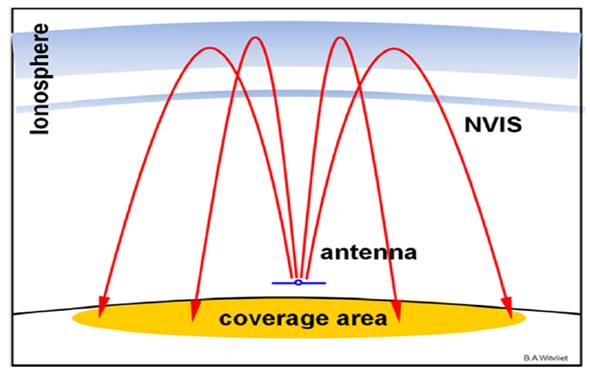
\includegraphics[width=0.6\textwidth]{bilder/NVIS-Propagation}
%	\label{fig:nvis-propagation}
%	\caption{NVIS-utbredning, princip}
%\end{figure}

NVIS används mycket på t.ex. 80-metersbandet för olika ''ringar'' och liknande när man träffas flera sändaramatörer på en viss frekvens en viss tid och sedan turas om att sända och kommentera på olika saker. 

\subsubsection{DX -- långväga kontakter}

För mer långväga kontakter lägger vi oss så högt det går, har antenner som sänder i en flackare vinkel, nästan rakt mot horisonten på lite högre höjd om möjligt och gärna också riktantenner i stället för de vanliga dipolerna som är den vanligaste antennen för de lägre kortvågsbanden.

Genom att kombinera detta och reflektera så högt upp i jonosfären som möjligt kan vi ibland nå mycket långt. Är konditionerna goda kan man få flera sådana hopp (skip) efter varandra och på så vis kan vi nå till andra sidan planeten. Vid gynnsamma konditioner kan man med relativt enkla medel prata med Japan och Australien på kortvåg.

\subsection{Bandens olika egenskaper}

\todo{Beskriva}

\subsubsection{160--80 meter}
\todo{Beskriva}


\subsubsection{40-60 meter}
\todo{Beskriva}

\subsubsection{20, 17, 12 och 10 meter}
\todo{Beskriva}



\begin{landscape}
\section{Frekvenser Amatörradio LF/MF/HF}
\subsection{Bandplaner LF/MF/HF}
Alla frekvenser i kHz, bandbredder i Hz.

\subsubsection{Bandplan 2.2\,km, 135,7--137,8\,kHz}
\begin{tabular}{rrrll}
\textbf{Frekvens} &  & \textbf{BW} & \textbf{Trafik} & \textbf{Noteringar} \\ \hline
135,7 & 135,8 & 200 & CQ, QRSS, Digi & OBS! Högsta effekt 1W ERP. \\ \hline
\end{tabular}

\subsubsection{Bandplan 600\,m, 472--479\,kHz}
\begin{tabular}{rrrll}
\multicolumn{2}{c}{\textbf{Frekvens}} & \textbf{BW} & \textbf{Trafik} & \textbf{Noteringar} \\ \hline
472 & 479 & 200 & CW, QRSS, Digi & OBS! Högsta utstrålad effekt 1W EIRP \\ \hline
\end{tabular}

\subsubsection{Bandplan 160\,m, 1810--2000\,kHz}
\begin{tabular}{rrrll}
\multicolumn{2}{c}{\textbf{Frekvens}} & \textbf{BW} & \textbf{Trafik} & \textbf{Noteringar} \\ \hline
1 810 & 1 838 & 200  & CW         & Exklusivt för CW. Interkontinental trafik har prio. \\ \hline
1 838 & 1 840 & 500  & Smalband   & Ej packet på 160m, PSK 1 838,150                    \\ \hline
1 840 & 1 850 & 2700 & Alla moder & Även digimode. SSB QRP 1 843 kHz                    \\ \hline
1 850 & 1 900 & 2700 & Alla moder & OBS! Max 10 W till ant.                             \\ \hline
1 900 & 1 950 & 2700 & Alla moder & OBS! Max 100 W till ant.                            \\ \hline
1 950 & 2 000 & 2700 & Alla moder & OBS! Max 10 W till ant.                             \\ \hline
\end{tabular}

\subsubsection{Bandplan 80\,m, 3500--3800\,kHz}
\begin{tabular}{rrrll}
\multicolumn{2}{c}{\textbf{Frekvens}} & \textbf{BW} & \textbf{Trafik} & \textbf{Noteringar} \\ \hline
3 500 & 3 510 & 200  & CW             & Exklusivt CW                         \\ 
      &       &      &                & Interkontinental DX-trafik har prio  \\ \hline
3 510 & 3 580 & 200  & CW             & Exklusivt CW contest 3510-–560       \\ 
      &       &      &                & CW QRS 3 555 kHz, CW QRP 3 560       \\ \hline
3 580 & 3 600 & 500  & Smalband, Digi & PSK 3 580,150                        \\
      &       &      &                & Automatiska Digimoder 3 590--600     \\ \hline
3 600 & 3 620 & 2700 & Alla moder     & Digimoder Automatiska Digimoder      \\ \hline
3 600 & 3 650 & 2700 & Alla moder     & SSB contest 3 600--650               \\
      &       &      &                & DV 3 630                             \\ \hline
3 650 & 3 700 & 2700 & Alla moder     & SSB QRP 3 690                        \\ \hline
3 700 & 3 800 & 2700 & Alla moder     & Contest 3 700-–800                   \\
      &       &      &                & Image 3 775                          \\
      &       &      &                & Region 1 nödfrekvens 3 760           \\ \hline
3 775 & 3 800 & 2700 & Alla moder     & Interkontinental DX-trafik prioritet \\ \hline
\end{tabular}

\subsubsection{Bandplan 40\,m, 7000--7200\,kHz}
\begin{tabular}{rrrll}
\multicolumn{2}{c}{\textbf{Frekvens}} & \textbf{BW} & \textbf{Trafik} & \textbf{Noteringar} \\ \hline
7\,000 & 7\,040 & 200  & CW         & Exklusivt CW.                             \\
      &       &      &            & QRP aktivitetscentrum 7\,030\,kHz           \\ \hline
7\,040 & 7\,050 & 500  & Smalband   & Digimoder Automatiska inom 7\,047–-050\,kHz \\ \hline
7\,050 & 7\,060 & 2700 & Alla moder & Digimoder Automatiska inom 7\,050–-053\,kHz \\ \hline
7\,060 & 7\,100 & 2700 & Alla moder & SSB contest i segmentet                   \\
      &       &      &            & DV 7 070 kHz, SSB QRP 7\,090 kHz           \\ \hline
7\,100 & 7\,130 & 2700 & Alla moder & Region 1 nödfrekvens 7\,110 kHz            \\ \hline
7\,130 & 7\,200 & 2700 & Alla moder & SSB contest i segmentet                   \\
      &       &      &            & Image 7\,165\,kHz                           \\ \hline
7\,175 & 7\,200 & 2700 & Alla moder & Interkontinental DX-trafik prio           \\ \hline
\end{tabular}

\subsubsection{Bandplan 30 m, 10100--10150 kHz}
\begin{tabular}{rrrll}
\multicolumn{2}{c}{\textbf{Frekvens}} & \textbf{BW} & \textbf{Trafik} & \textbf{Noteringar} \\ \hline
10\,100 & 10\,140 & 200 & CW       & CW exkl. Max 150 Watt på 30 m    \\
       &        &     &          & CW QRP 10\,116\,kHz                     \\ \hline
10\,140 & 10\,150 & 500 & Smalband & Digimoder PSK 10142,150\,kHz. Ej Packet \\ \hline
\end{tabular}

\subsubsection{Bandplan 20 m, 14000--14350 kHz}
\begin{tabular}{rrrll}
\multicolumn{2}{c}{\textbf{Frekvens}} & \textbf{BW} & \textbf{Trafik} & \textbf{Noteringar} \\ \hline
14\,000 & 14\,070 & 200  & CW         & Exklusivt CW                            \\
       &        &      &            & Conctest 14\,000-–060                     \\
       &        &      &            & CW QRS 14 055, CW QRP 14\,060            \\ \hline
14\,070 & 14\,099 & 500  & Smalband   & PSK 14 070,150                          \\
       &        &      &            & Auto Digimoder 14 089-–099              \\ \hline
14\,099 & 14\,101 & 200  & Fyrar      & Exklusivt IBP, endast fyrar             \\ \hline
14\,101 & 14 \,12 & 2700 & Alla moder & Digitala moder och obevakade Digimoder  \\ \hline
14\,112 & 14\,350 & 2700 & Alla moder & SSB Contest 14 125--300                 \\
       &        &      &            & DV 14 130, DXpedition prio 14\,195$\pm$5 \\ \hline
14\,300 & 14\,350 & 2700 & Alla moder & Image 14\,230, SSB QRP 14\,285            \\
       &        &      &            & Global nödfrekvens 14 300               \\ \hline
\end{tabular}

\subsubsection{Bandplan 17 m, 18068--18168 kHz}
\begin{tabular}{rrrll}
\multicolumn{2}{c}{\textbf{Frekvens}} & \textbf{BW} & \textbf{Trafik} & \textbf{Noteringar} \\ \hline
18 068 & 18 095 & 200  & CW         & CW exklusivt. QRP 18 086             \\ \hline
18 095 & 18 109 & 500  & Smalband   & Digimoder PSK 18 100,150             \\
       &        &      &            & Automatiska Digimoder 18 105-–18 109 \\ \hline
18 109 & 18 111 & 200  & Fyrar      & Exklusivt fyrar, IBP fyrnät          \\ \hline
18 111 & 18 168 & 2700 & Alla moder & Digi 18 111–-18 120                  \\
       &        &      &            & SSB QRP 18 130, DV 18 150            \\
       &        &      &            & Global nödfrekv. 18 160\\ \hline
\end{tabular}

\subsubsection{Bandplan 15 m, 21000--21450 kHz}
\begin{tabular}{rrrll}
\multicolumn{2}{c}{\textbf{Frekvens}} & \textbf{BW} & \textbf{Trafik} & \textbf{Noteringar} \\ \hline
21 000 & 21 070 & 200  & CW         & Exklusivt CW, QRS 21 055, CW QRP 21 060          \\ \hline
21 070 & 21 110 & 500  & Smalband   & PSK 21080.150, Automatiska Digimoder 21 090–-110 \\
21 110 & 21 120 & 2700 & Alla moder & Alla moder utom SSB!                             \\
       &        &      &            & Digimoder, och Automatiska Digimoder             \\ \hline
21 120 & 21 149 & 500  & Smalband   &                                                  \\ \hline
21 149 & 21 151 & 200  & Fyrar      & Exklusivt fyrar. IBP fyrnät                      \\ \hline
21 151 & 21 450 & 2700 & Alla moder & DV 21 180, SSB QRP 21 285, Image 21 340          \\
       &        &      &            & Global nödfrekv. 21 360                          \\ \hline
\end{tabular}

\subsubsection{Bandplan 12 m, 24890--24990 kHz}
\begin{tabular}{rrrll}
\multicolumn{2}{c}{\textbf{Frekvens}} & \textbf{BW} & \textbf{Trafik} & \textbf{Noteringar} \\ \hline
24 890 & 24 915 & 200  & CW         & Exklusivt CW, QRP 24 906                             \\ \hline
24 915 & 24 929 & 500  & Smalband   & PSK 24 920.150, Automatiska Digimoder 24 925–-24 929 \\ \hline
24 929 & 24 931 & 200  & Fyrar      & Fyrar, IBP fyrnät                                    \\ \hline
24 931 & 24 990 & 2700 & Alla moder & Auto Digimoder 24 931-–24 940                        \\
       &        &      &            & SSB QRP 24 950, DV 24 960                            \\ \hline
\end{tabular}

\subsubsection{Bandplan 10 m, 28000-29700 kHz}
\begin{tabular}{rrrll}
\multicolumn{2}{c}{\textbf{Frekvens}} & \textbf{BW} & \textbf{Trafik} & \textbf{Noteringar} \\ \hline
28 000 & 28 070 & 200  & CW         & Exklusivt CW, QRS 28 055, CW QRP 28 060                \\ \hline
28 070 & 28 190 & 500  & Smalband   & PSK 28 120.150, Auto Digimoder inom 28 120--150        \\ \hline
28 190 & 28 199 & 200  & Fyrar IBP  & Regionala fyrar med tidsdelning                        \\ \hline
28 199 & 28 201 & 200  & Fyrar IBP  & IBP fyrnät                                             \\ \hline
28 201 & 28 225 & 200  & Fyrar IBP  & kontinuerligt sändande fyrar                           \\ \hline
28 225 & 28 300 & 2700 & Alla moder & Övriga fyrar                                           \\ \hline
28 300 & 28 320 & 2700 & Alla moder & Digimoder och Automatiska Digimoder                    \\ \hline
28 320 & 29 100 & 2700 & Alla moder & DV 28 330 kHz, SSB QRP 28 360 kHz                      \\
       &        &      &            & Image 28 680 kHz                                       \\ \hline
29 100 & 29 200 & 6000 & Alla moder & FM simplex, 10 kHz kanaler                             \\
       &        &      &            & Maximalt ±2.5 kHz dev., max 2.5 kHz mod.frek.          \\ \hline
29 200 & 29 300 & 6000 & Alla moder & Digimoder och Automatiska Digimoder                    \\ \hline
29 300 & 29 510 & 6000 & Satellit   & Nerlänk fr. satellit. EJ SÄNDNING I SEGMENTET          \\ \hline
29 510 & 29 520 & 6000 & Skydd      & Skyddsfrekvens för satelliter. EJ SÄNDNING I SEGMENTET \\ \hline
29 520 & 29 590 & 6000 & Alla moder & FM Repeater in RH1--8, 100 kHz duplex, 2.5 kHz NBFM    \\ \hline
29 600 & 29 620 & 6000 & Alla moder & FM simplex, anrop 29 600                               \\
       &        &      &            & FM simplex repeater 29 610                             \\ \hline
29 620 & 29 700 & 6000 & Alla moder & FM Repeater ut RH1--8, 100 kHz duplex                  \\ \hline
\end{tabular}
\end{landscape}

\clearpage

%\small
%\begin{landscape}
%\subsection{PTS Bandplan för VLF, 3-30 kHz}
%\begin{longtable}{lll}
%\textbf{Frekvens} & \textbf{Användning}              & \textbf{Anmärkning}             \\ \hline \endhead
%0,009--0,014	 & Radionavigering                 & Sjöfart  \\	 
%0,009--0,014	 & Radionavigering                 & Luftfart \\	 
%0,009--0,01995	 & Militär användning              &          \\
%0,014--0,01995	 & Fast radio                      &          \\
%0,014--0,01995	 & Sjöfartsradio                   &          \\
%0,01995--0,02005 & Standardfrekvens och tidssignal &          \\ 
%\end{longtable}
%
%\subsection{PTS Bandplan för LF, 30-300 kHz}
%\begin{longtable}{lll}
%\textbf{Frekvens} & \textbf{Användning}  & \textbf{Anmärkning}                     \\ \hline \endhead
%0,1176--0,126     & Militär användning   &                                         \\
%0,1176--0,126     & Sjöfartsradio        &                                         \\
%0,129--0,1485     & Militär användning   &                                         \\
%0,129--0,1485     & Sjöfartsradio        &                                         \\
%0,1357--0,1378    & \textbf{Amatörradio} & Undantag från tillståndsplikt (Max 1 W) \\
%0,1485--0,2835    & Rundradio            & GE75                                    \\
%\end{longtable}
%
%\subsection{PTS Bandplan för MF, 300-3000 kHz}
%\begin{longtable}{lll}
%\textbf{Frekvens} & \textbf{Användning}              & \textbf{Anmärkning}             \\ \hline \endhead
%
%0,315--0,6	 & Djurimplantat                   & Undantag från tillståndsplikt             \\
%0,4--0,6	 & RFID                            & Undantag från tillståndsplikt             \\
%0,405--0,415	 & Militär användning              &                                           \\	 
%0,4065--0,4135	 & Radionavigering                 & Sjöfart                                   \\
%0,415--0,435	 & Radionavigering                 & Luftfart GE85M                            \\
%0,415--0,435	 & Militär användning              & GE85M                                     \\
%0,415--0,495	 & Sjöfartsradio                   & GE85M                                     \\
%0,415--0,435	 & Radiofyrar                      & Luftfart	GE85M                          \\
%0,435--0,5265	 & Militär användning              &                                           \\ 
%0,4569--0,4571	 & Lokalisering av nödställda      & Undantag från tillståndsplikt             \\
%0,472--0,479	 & \textbf{Amatörradio}            & Undantag från tillståndsplikt (Max 1 W)   \\
%0,495--0,5265	 & Sjöfartsradio                   &                                           \\
%0,495--0,505	 & Luftfartsradio                  &                                           \\
%0,51775--0,51825 & Sjöfartsradio                   & NAVTEX                                    \\
%0,5265--1,6065	 & Rundradio                       & GE75                                      \\
%1,6065--1,625	 & Militär användning              & GE85M                                     \\
%1,6065--1,625	 & Sjöfartsradio                   & GE85M                                     \\
%1,625--1,635	 & Militär användning              &                                           \\
%1,625--1,635	 & Radiolokalisering               &                                           \\
%1,635--1,8	 & Militär användning              & GE85M                                     \\
%1,635--1,8	 & Sjöfartsradio                   & GE85M                                     \\
%1,8--1,81	 & Militär användning              &                                           \\ 
%1,8--1,81	 & Radiolokalisering               &                                           \\
%1,81--1,85	 & \textbf{Amatörradio}            & Undantag från tillståndsplikt             \\
%1,85--2,045	 & Militär användning              &                                           \\
%1,85--2,045	 & Fast radio                      &                                           \\
%1,85--2,045	 & Sjöfartsradio                   &                                           \\
%1,85--2	 	 & \textbf{Amatörradio}            & Undantag från tillståndsplikt (Max 10 W)  \\
%1,85--2,045	 & Landmobil radio                 &                                           \\
%2,045--2,16	 & Militär användning              & GE85M                                     \\
%2,045--2,16	 & Sjöfartsradio                   & GE85M                                     \\
%2,16--2,1735	 & Militär användning              &                                           \\	 
%2,16--2,17	 & Radiolokalisering               &                                           \\	 
%2,17--2,1735	 & Sjöfartsradio                   &                                           \\
%2,1735--2,1905	 & Sjöfartsradio                   & Internationella nöd- och anropsfrekvenser \\
%                 &                                 & 2182 kHz (telefoni) och 2187,5 kHz (DSC)  \\
%2,1905--2,498	 & Militär användning              &                                           \\	 
%2,1905--2,498	 & Sjöfartsradio                   &                                           \\
%2,194--2,498	 & Fast radio                      &                                           \\
%2,194--2,498	 & Landmobil radio                 &                                           \\	 
%2,498--2,502	 & Standardfrekvens och tidssignal &                                           \\
%2,502--2,85	 & Militär användning              &                                           \\
%2,502--2,625	 & Fast radio                      &                                           \\
%2,502--2,85	 & Sjöfartsradio                   &                                           \\
%2,502--2,625	 & Landmobil radio                 &                                           \\	 
%2,625--2,65	 & Radionavigering för sjöfart     &                                           \\
%2,65--2,85	 & Fast radio                      &                                           \\
%2,65--2,85	 & Landmobil radio                 &                                           \\	 
%\end{longtable}
%
%\subsection{PTS Bandplan för HF, 3-30 MHz}
%\begin{longtable}{lll}
%\textbf{Frekvens} & \textbf{Användning}              & \textbf{Anmärkning}             \\ \hline \endhead
%3,0215--3,0245    & Sjöfartsradio                    & Nöd- och säkerhetstrafik        \\
%3,025--3,155      & Militär användning               & RR AP26                         \\
%3,025--3,155      & Luftfartsradio                   & RR AP26                         \\
%3,155--3,4        & Militär användning               &                                 \\
%3,155--3,4        & Induktiva tillämpningar          & Undantag från tillståndsplikt   \\ 
%                  &                                  & 2006/771/EG 2013/752/EU         \\
%3,155--3,4        & Fast radio                       &                                 \\
%3,155--3,4        & Sjöfartsradio                    &                                 \\
%3,155--3,4        & Landmobil radio                  &                                 \\
%3,4--3,5          & Luftfartsradio                   & RR AP27                         \\
%3,5--3,9          & Militär användning               &                                 \\	 
%3,5--3,9          & Fast radio                       &                                 \\
%3,5--3,8          & Sjöfartsradio                    &                                 \\
%3,5--3,8          & \textbf{Amatörradio}             & \textbf{80-metersbandet}        \\
%3,5--3,9          & Landmobil radio                  &                                 \\
%3,8--3,9          & Luftfartsradio                   &                                 \\
%3,9--3,95         & Militär användning               & RR AP26                         \\
%3,9--3,95         & Luftfartsradio                   & RR AP26                         \\
%3,95--4,995       & Militär användning               &                                 \\
%3,95--4,063       & Fast radio                       &                                 \\	 
%3,95--4           & Rundradio                        &                                 \\
%4--4,063          & Sjöfartsradio                    & Radiotelefoni                   \\
%4,063--4,438      & Sjöfartsradio                    & RR AP25 gäller i del av bandet  \\
%4,438--4,65       & Fast radio                       &                                 \\
%4,438--4,65       & Sjöfartsradio                    &                                 \\
%4,438--4,65       & Landmobil radio                  &                                 \\
%4,65--4,7         & Luftfartsradio                   & RR AP27                         \\
%4,7--4,75         & Luftfartsradio                   & RR AP26                         \\
%4,75--4,995       & Fast radio                       &                                 \\
%4,75--4,85        & Luftfartsradio                   &                                 \\
%4,75--4,995       & Landmobil radio                  &                                 \\
%4,995--5,005      & Fyr                              & Standardfrekvens och tidssignal \\
%5,005--5,9        & Militär användning               &                                 \\
%5,005--5,48       & Fast radio                       &                                 \\
%5,06--5,45        & Sjöfartsradio                    &                                 \\
%5,06--5,48        & Landmobil radio                  &                                 \\
%5,45--5,48        & Luftfartsradio                   &                                 \\
%5,48--5,68        & Luftfartsradio                   & RR AP27                         \\
%5,6785--5,6815    & Sjöfartsradio                    & Nöd- och säkerhetstrafik.       \\
%5,68--5,73        & Luftfartsradio                   & RR AP26                         \\
%5,73--5,9         & Fast radio                       &                                 \\
%5,73--5,9         & Landmobil radio                  &                                 \\
%5,9--6,2          & Rundradio                        &                                 \\
%6,2--6,525        & Militär användning               & RR AP25 gäller i del av bandet  \\
%6,2--6,525        & Sjöfartsradio                    & RR AP25 gäller i del av bandet  \\
%6,525--7          & Militär användning               &                                 \\
%6,525--6,685      & Luftfartsradio                   & RR AP27                         \\
%6,685--6,765      & Luftfartsradio                   & RR AP26                         \\
%6,765--6,795      & Induktiva tillämpningar          & Undantag från tillståndsplikt   \\
%6,765--7          & Fast radio                       &                                 \\
%6,765--7          & Landmobil radio                  &                                 \\
%6,765--6,795      & Allmän kortdistansradio          & Undantag från tillståndsplikt   \\
%7--7,2            & \textbf{Amatörradio}             & \textbf{40-metersbandet}        \\
%7,2--7,45         & Rundradio                        &                                 \\
%7,4--8,8          & Induktiva tillämpningar          & Undantag från tillståndsplikt   \\
%7,45--9,4         & Militär användning               &                                 \\
%7,45--8,195       & Fast radio                       &                                 \\
%7,45--8,1         & Landmobil radio                  &                                 \\
%8,1--8,195        & Sjöfartsradio                    &                                 \\
%8,195--8,815      & Sjöfartsradio                    & RR AP25 gäller i del av bandet  \\
%8,815--8,965      & Luftfartsradio                   & RR AP27                         \\
%8,965--9,04       & Luftfartsradio                   & RR AP26                         \\
%9,04--9,4         & Fast radio                       &                                 \\
%9,4--9,9          & Rundradio                        &                                 \\
%9,9--9,995        & Militär användning               &                                 \\
%9,9--9,995        & Fast radio                       &                                 \\
%9,995--10,005     & Standardfrekvens och tidssignal  &                                 \\
%10,005--10,1      & Luftfartsradio                   & RR AP27                         \\
%10,1--11,175      & Militär användning               &                                 \\
%10,1--11,175      & Fast radio                       &                                 \\
%10,1--10,15       & \textbf{Amatörradio}             & \textbf{30-metersbandet}        \\
%10,15--11,175     & Sjöfartsradio                    &                                 \\
%10,15--11,175     & Landmobil radio                  &                                 \\
%10,2--11          & Induktiva tillämpningar          & Undantag från tillståndsplikt   \\
%11,175--11,275    & Luftfartsradio                   & RR AP26                         \\
%11,275--11,4      & Luftfartsradio                   & RR AP27                         \\
%11,4--11,6        & Militär användning               &                                 \\
%11,4--11,6        & Fast radio                       &                                 \\
%11,6--12,1        & Rundradio                        &                                 \\
%12,1--12,23       & Militär användning               &                                 \\
%12,1--12,23       & Fast radio                       &                                 \\
%12,23--13,2       & Militär användning               & RR AP25 gäller i del av bandet  \\
%12,23--13,2       & Sjöfartsradio                    & RR AP25 gäller i del av bandet  \\
%12,5--20          & Djurimplantat                    & Undantag från tillståndsplikt   \\
%13,2--13,57       & Militär användning               &                                 \\
%13,2--13,26       & Luftfartsradio                   & RR AP26                         \\
%13,26--13,36      & Luftfartsradio                   & RR AP27                         \\
%13,36--13,57      & Fast radio                       &                                 \\
%13,36--13,41      & Radioastronomi                   & Onsala rymd - observatorium     \\
%13,41--13,57      & Sjöfartsradio                    &                                 \\
%13,41--13,57      & Landmobil radio                  &                                 \\
%13,553--13,567    & Induktiva tillämpningar          & Undantag från tillståndsplikt   \\
%13,553--13,567    & RFID                             & Undantag från tillståndsplikt   \\
%13,553--13,567    & Allmän kortdistansradio          & Undantag från tillståndsplikt   \\
%13,553--13,567    & ISM                              &                                 \\
%13,57--13,87      & Rundradio                        &                                 \\
%13,87--14         & Militär användning               &                                 \\
%13,87--14         & Fast radio                       &                                 \\
%13,87--14         & Sjöfartsradio                    &                                 \\
%13,87--14         & Landmobil radio                  &                                 \\
%14--14,35         & \textbf{Amatörradio}             & \textbf{20-metersbandet}        \\
%14,35--14,99      & Militär användning               &                                 \\
%14,35--14,99      & Fast radio                       &                                 \\
%14,35--14,99      & Sjöfartsradio                    &                                 \\
%14,35--14,99      & Landmobil radio                  &                                 \\
%14,99--15,01      & Standardfrekvens och tidssignal  &                                 \\
%15,01--15,1       & Militär användning               &                                 \\
%15,01--15,1       & Luftfartsradio                   & RR AP26                         \\
%15,1--15,8        & Rundradio                        &                                 \\
%15,8--16,36       & Militär användning               &                                 \\
%15,8--16,36       & Fast radio                       &                                 \\
%16,36--17,41      & Militär användning               & RR AP25 gäller i del av bandet  \\
%16,36--17,41      & Sjöfartsradio                    & RR AP25 gäller i del av bandet  \\
%17,41--17,48      & Militär användning               &                                 \\
%17,41--17,48      & Fast radio                       &                                 \\
%17,48--17,9       & Rundradio                        &                                 \\
%17,9--17,97       & Luftfartsradio                   & RR AP27                         \\
%17,97--18,068     & Militär användning               &                                 \\
%17,97--18,03      & Luftfartsradio                   & RR AP26                         \\
%18,03--18,068     & Fast radio                       &                                 \\
%18,068--18,168    & \textbf{Amatörradio}             & \textbf{17-metersbandet}        \\
%18,168--18,78     & Militär användning               &                                 \\
%18,168--18,78     & Fast radio                       &                                 \\
%18,168--18,78     & Sjöfartsradio                    &                                 \\
%18,168--18,78     & Landmobil radio                  &                                 \\
%18,78--18,9       & Militär användning               & RR AP25 gäller i del av bandet  \\
%18,78--18,9       & Sjöfartsradio                    & RR AP25 gäller i del av bandet  \\
%18,9--19,02       & Rundradio                        &                                 \\
%19,02--19,68      & Militär användning               &                                 \\
%19,02--19,68      & Fast radio                       &                                 \\
%19,68--19,8       & Militär användning               & RR AP25 gäller i del av bandet  \\
%19,68--19,8       & Sjöfartsradio                    & RR AP25 gäller i del av bandet  \\
%19,8--19,99       & Militär användning               &                                 \\
%19,8--19,99       & Fast radio                       &                                 \\
%19,99--20,01      & Standardfrekvens och tidssignal  &                                 \\
%20,01--21         & Militär användning               &                                 \\
%20,01--21         & Fast radio                       &                                 \\
%20,01--21         & Landmobil radio                  &                                 \\
%21--21,45         & \textbf{Amatörradio}             & \textbf{14-metersbandet}        \\
%21,45--21,85      & Rundradio                        &                                 \\
%21,85--21,924     & Militär användning               &                                 \\
%21,85--21,924     & Fast radio                       &                                 \\
%21,924--22        & Luftfartsradio                   & RR AP27 gäller i del av bandet  \\
%22--22,855        & Militär användning               & RR AP25 gäller i del av bandet  \\
%22--22,855        & Sjöfartsradio                    & RR AP25 gäller i del av bandet  \\
%22,855--24,89     & Militär användning               &                                 \\
%22,855--24,89     & Fast radio                       &                                 \\
%23--23,2          & Sjöfartsradio                    &                                 \\
%23--23,2          & Landmobil radio                  &                                 \\
%23,2--23,35       & Luftfartsradio                   &                                 \\
%23,35--24         & Sjöfartsradio                    &                                 \\
%23,35--24         & Landmobil radio                  &                                 \\
%24,89--24,99      & \textbf{Amatörradio}             & \textbf{12-metersbandet}        \\
%24,99--25,01      & Standardfrekvens och tidssignal  &                                 \\
%25,01--25,55      & Militär användning               &                                 \\
%25,01--25,07      & Fast radio                       &                                 \\
%25,01--25,07      & Sjöfartsradio                    &                                 \\
%25,01--25,07      & Landmobil radio                  &                                 \\
%25,07--25,21      & Sjöfartsradio (GMDSS)            & RR AP25 gäller i del av bandet  \\
%25,21--25,55      & Fast radio                       &                                 \\
%25,21--25,55      & Sjöfartsradio                    &                                 \\
%25,21--25,55      & Landmobil radio                  &                                 \\
%25,55--25,67      & Radioastronomi                   & Onsala rymd - observatorium     \\
%25,67--26,1       & Rundradio                        &                                 \\
%26,1--26,175      & Militär användning               & RR AP25 gäller i del av bandet  \\
%26,1--26,175      & Sjöfartsradio                    & RR AP25 gäller i del av bandet  \\
%26,175--28        & Militär användning               &                                 \\
%26,175--27,5      & Fast radio                       &                                 \\
%26,175--28        & Landmobil radio                  &                                 \\
%26,175--27,5      & Personsökning                    &                                 \\
%26,82--27,2       & Telemetri och radiostyrning      & Undantag från tillståndsplikt   \\
%26,85--26,86      & Larmöverföring                   & Undantag från tillståndsplikt   \\
%26,957--27,283    & Induktiva tillämpningar          & Undantag från tillståndsplikt   \\
%                  &                                  & 2006/771/EG 2013/752/EU         \\
%26,957--27,2      & Allmän kortdistansradio          & Undantag från tillståndsplikt   \\
%                  &                                  & 2006/771/EG 2013/752/EU         \\
%26,957--27,283    & ISM                              &                                 \\
%26,96--27,41      & \textbf{Privatradio (CB 27 MHz)} & Undantag från tillståndsplikt   \\
%26,99--27,2       & Trådlösa barnvaktssystem         & Undantag från tillståndsplikt   \\
%28--29,7          & \textbf{Amatörradio}             & \textbf{10-metersbandet}        \\
%\end{longtable}
%\normalsize
%\end{landscape}

%\begin{landscape}
\section{Logbook}
\begin{longtable}{|c|c|c|c|c|c|c|c|c|c|}
	\hline
	Station  & Datum  & \multicolumn{2}{|c|}{Tid UTC} & Frekvens & Mode & Effekt & \multicolumn{2}{|c|}{Rapport} & Noteringar / QSL mm \\
	 Signal  & YYMMDD & HHMM &          HHMM          & MHz/kHz  &      & dBm/W  & RX &            TX            &  \\ \hline
	\endhead &        &      &                        &          &      &        &    &                          &  \\ \hline
	         &        &      &                        &          &      &        &    &                          &  \\ \hline
	         &        &      &                        &          &      &        &    &                          &  \\ \hline
	         &        &      &                        &          &      &        &    &                          &  \\ \hline
	         &        &      &                        &          &      &        &    &                          &  \\ \hline
	         &        &      &                        &          &      &        &    &                          &  \\ \hline
	         &        &      &                        &          &      &        &    &                          &  \\ \hline
	         &        &      &                        &          &      &        &    &                          &  \\ \hline
	         &        &      &                        &          &      &        &    &                          &  \\ \hline
	         &        &      &                        &          &      &        &    &                          &  \\ \hline
	         &        &      &                        &          &      &        &    &                          &  \\ \hline
	         &        &      &                        &          &      &        &    &                          &  \\ \hline
	         &        &      &                        &          &      &        &    &                          &  \\ \hline
	         &        &      &                        &          &      &        &    &                          &  \\ \hline
	         &        &      &                        &          &      &        &    &                          &  \\ \hline
	         &        &      &                        &          &      &        &    &                          &  \\ \hline
	         &        &      &                        &          &      &        &    &                          &  \\ \hline
	         &        &      &                        &          &      &        &    &                          &  \\ \hline
	         &        &      &                        &          &      &        &    &                          &  \\ \hline
	         &        &      &                        &          &      &        &    &                          &  \\ \hline
	         &        &      &                        &          &      &        &    &                          &  \\ \hline
	         &        &      &                        &          &      &        &    &                          &  \\ \hline
	         &        &      &                        &          &      &        &    &                          &  \\ \hline
	         &        &      &                        &          &      &        &    &                          &  \\ \hline
	         &        &      &                        &          &      &        &    &                          &  \\ \hline
	         &        &      &                        &          &      &        &    &                          &  \\ \hline
	         &        &      &                        &          &      &        &    &                          &  \\ \hline
	         &        &      &                        &          &      &        &    &                          &  \\ \hline
	         &        &      &                        &          &      &        &    &                          &  \\ \hline
	         &        &      &                        &          &      &        &    &                          &  \\ \hline
	         &        &      &                        &          &      &        &    &                          &  \\ \hline
	         &        &      &                        &          &      &        &    &                          &  \\ \hline
	         &        &      &                        &          &      &        &    &                          &  \\ \hline
	         &        &      &                        &          &      &        &    &                          &  \\ \hline
	         &        &      &                        &          &      &        &    &                          &  \\ \hline
	         &        &      &                        &          &      &        &    &                          &  \\ \hline
	         &        &      &                        &          &      &        &    &                          &  \\ \hline
	         &        &      &                        &          &      &        &    &                          &  \\ \hline
	         &        &      &                        &          &      &        &    &                          &  \\ \hline
	         &        &      &                        &          &      &        &    &                          &  \\ \hline
	         &        &      &                        &          &      &        &    &                          &  \\ \hline
	         &        &      &                        &          &      &        &    &                          &  \\ \hline
	         &        &      &                        &          &      &        &    &                          &  \\ \hline
	         &        &      &                        &          &      &        &    &                          &  \\ \hline
	         &        &      &                        &          &      &        &    &                          &  \\ \hline
	         &        &      &                        &          &      &        &    &                          &  \\ \hline
	         &        &      &                        &          &      &        &    &                          &  \\ \hline
	         &        &      &                        &          &      &        &    &                          &  \\ \hline
	         &        &      &                        &          &      &        &    &                          &  \\ \hline
	         &        &      &                        &          &      &        &    &                          &  \\ \hline
	         &        &      &                        &          &      &        &    &                          &  \\ \hline
	         &        &      &                        &          &      &        &    &                          &  \\ \hline
	         &        &      &                        &          &      &        &    &                          &  \\ \hline
	         &        &      &                        &          &      &        &    &                          &  \\ \hline
	         &        &      &                        &          &      &        &    &                          &  \\ \hline
	         &        &      &                        &          &      &        &    &                          &  \\ \hline
	         &        &      &                        &          &      &        &    &                          &  \\ \hline
	         &        &      &                        &          &      &        &    &                          &  \\ \hline
	         &        &      &                        &          &      &        &    &                          &  \\ \hline
	         &        &      &                        &          &      &        &    &                          &  \\ \hline
	         &        &      &                        &          &      &        &    &                          &  \\ \hline
	         &        &      &                        &          &      &        &    &                          &  \\ \hline
	         &        &      &                        &          &      &        &    &                          &  \\ \hline
	         &        &      &                        &          &      &        &    &                          &  \\ \hline
	         &        &      &                        &          &      &        &    &                          &  \\ \hline
	         &        &      &                        &          &      &        &    &                          &  \\ \hline
	         &        &      &                        &          &      &        &    &                          &  \\ \hline
	         &        &      &                        &          &      &        &    &                          &  \\ \hline
	         &        &      &                        &          &      &        &    &                          &  \\ \hline
	         &        &      &                        &          &      &        &    &                          &  \\ \hline
	         &        &      &                        &          &      &        &    &                          &  \\ \hline
	         &        &      &                        &          &      &        &    &                          &  \\ \hline
	         &        &      &                        &          &      &        &    &                          &  \\ \hline
	         &        &      &                        &          &      &        &    &                          &  \\ \hline
	         &        &      &                        &          &      &        &    &                          &  \\ \hline
	         &        &      &                        &          &      &        &    &                          &  \\ \hline
	         &        &      &                        &          &      &        &    &                          &  \\ \hline
	         &        &      &                        &          &      &        &    &                          &  \\ \hline
	         &        &      &                        &          &      &        &    &                          &  \\ \hline
	         &        &      &                        &          &      &        &    &                          &  \\ \hline
	         &        &      &                        &          &      &        &    &                          &  \\ \hline
	         &        &      &                        &          &      &        &    &                          &  \\ \hline
	         &        &      &                        &          &      &        &    &                          &  \\ \hline
	         &        &      &                        &          &      &        &    &                          &  \\ \hline
	         &        &      &                        &          &      &        &    &                          &  \\ \hline
	         &        &      &                        &          &      &        &    &                          &  \\ \hline
	         &        &      &                        &          &      &        &    &                          &  \\ \hline
	         &        &      &                        &          &      &        &    &                          &  \\ \hline
	         &        &      &                        &          &      &        &    &                          &  \\ \hline
	         &        &      &                        &          &      &        &    &                          &  \\ \hline
	         &        &      &                        &          &      &        &    &                          &  \\ \hline
	         &        &      &                        &          &      &        &    &                          &  \\ \hline
	         &        &      &                        &          &      &        &    &                          &  \\ \hline
	         &        &      &                        &          &      &        &    &                          &  \\ \hline
	         &        &      &                        &          &      &        &    &                          &  \\ \hline
	         &        &      &                        &          &      &        &    &                          &  \\ \hline
	         &        &      &                        &          &      &        &    &                          &  \\ \hline
\end{longtable}
\end{landscape}
\clearpage


\end{document}
